\chapter{Formulating Auxiliary Field Quantum Monte Carlo}
\label{ap:theoAFQMC}

%\pagebreak

\section{Casting the fermionic trace as a determinant}\label{sec:trace_det}

Let the two arbitrary real matrices be $\bm M$ and $\bm N$.
Then, a particular case of the identity (\ref{eq:quadraticIdentity}) is
\begin{equation}\label{eq:particularIdentity}
\Tr \big[ e^{-c_i^\dagger M_{ij} c_j} e^{-c_i^\dagger N_{ij} c_j} \big] = \text{det} ( \bm I + e^{-{\bm M}} e^{-{\bm N}} ) ,
\end{equation}
where a summation over repeated indices is implied, as it wil be throughout this proof.

To prove this identity, we start by proving that
\begin{equation}\label{eq:identity_prod_exps}
e^{-c_i^\dagger M_{ij} c_j}  e^{-c_i^\dagger N_{ij} c_j} = e^{-\sum_\nu c_\nu^\dagger \rho_\nu c_\nu} ,
\end{equation}
where $\lambda_\nu = e^{-\rho_\nu}$ are the eigenvalues of the matrix $e^{-{\bm M}} e^{-{\bm N}}$.

The proof consists of showing that any many-particle state are propagated in the same way when acted upon by any of these two operators, i.e. the LHS operator leads the system to the same state as the RHS operator.

A generic single-particle state reads
\begin{equation}
\left| \phi \right\rangle = \sum_j a_j c_j^\dagger \left| 0 \right\rangle ,
\end{equation}
where $a_j$ are arbitrary coefficients, and $\left| 0 \right\rangle$ is the vacuum state.

Let $\{\left| \mu \right\rangle \}$ be the basis in which the matrix $\bm N$ is diagonal. Using Dirac notation, we then have
\begin{equation}
\bm N = \sum_{\mu} \left| \mu \right\rangle n_\mu \left\langle \mu \right|
\end{equation}

Define new fermionic operators
\begin{equation}\label{eq:changeBasis1}
c_\mu = \sum_j \left\langle \mu | j \right\rangle c_j \quad
c_\mu^\dagger = \sum_j \left\langle j | \mu \right\rangle c_j^\dagger ,
\end{equation}
which may be inverted to obtain
\begin{equation}\label{eq:changeBasis2}
c_j = \sum_\mu \left\langle j | \mu \right\rangle c_\mu \quad
c_j^\dagger = \sum_\mu \left\langle \mu | j \right\rangle c_\mu^\dagger ,
\end{equation}

Now we prove yet another identity that goes into proving equation (\ref{eq:identity_prod_exps}).
\begin{equation}\label{eq:LHS_identity}
e^{-c_i^\dagger N_{ij} c_j} = \prod_\mu \big[ \mathbbm{1} + ( e^{-n_\mu} - 1 ) c_\mu^\dagger c_\mu \big]
\end{equation}
\begin{equation*}
\begin{split}
&\exp({-c_i^\dagger N_{ij} c_j}) = \exp({ - \sum_{\mu\nu} \left\langle \mu | i \right\rangle c_\mu^\dagger N_{ij} \left\langle j | \nu \right\rangle c_\nu }) = \exp({-\sum_{ij}\sum_{ \mu\nu\sigma} \left\langle \mu | i \right\rangle  \left\langle i | \sigma \right\rangle c_\mu^\dagger n_\sigma \left\langle \sigma | j \right\rangle \left\langle j | \nu \right\rangle c_\nu }) , \\
& \text{(using the closure relation} \sum_i \left| i \right\rangle \left\langle i \right|= \mathbbm{1} \text{)} \\
&= \exp({-\sum_{ \mu\nu\sigma} \overbrace{\left\langle \mu | \sigma \right\rangle}^{\delta_{\mu\sigma}}  c_\mu^\dagger n_\sigma \overbrace{\left\langle \sigma | \nu \right\rangle}^{\delta_{\sigma\nu}} c_\nu }) = \exp({-\sum_\mu c_\mu^\dagger n_\mu c_\mu}) = \prod_\mu e^{-n_\mu \hat{n}_\mu} \\
&= \prod_\mu [ \mathbbm{1} + ( - n_\mu \hat{n}_\mu + \frac{n_\mu^2}{2!} \hat{n}_\mu^2 - \frac{n_\mu^3}{3!} \hat{n}_\mu^3 + ... ] = \prod_\mu [ \mathbbm{1} + ( - n_\mu + \frac{n_\mu^2}{2!} - \frac{n_\mu^3}{3!} + ... ) \hat{n}_\mu ] \\
& \text{(since  } \hat{n} = \hat{n}^k \text{  for all  } k \in \mathbb{N} \text{  for fermions since  } n = 0, 1 ) \\
&= \prod_\mu [ \mathbbm{1} + ( e^{-n_\mu} - 1 ) c_\mu^\dagger c_\mu ] \quad\quad \qedsymbol
\end{split}
\end{equation*}

Let 
$
\left| \phi \right\rangle = \sum_j a_j c_j^\dagger \left| 0 \right\rangle
$
be an arbitrary many-particle state. 

Now we use the previous identity to prove that applying the operator of equation (\ref{eq:LHS_identity}) to $\left| \phi \right\rangle$ we obtain
\begin{equation}
e^{-c_i^\dagger N_{ij} c_j} \left| \phi \right\rangle = \sum_j a_j' c_j^\dagger \left| 0 \right\rangle , 
\end{equation}
with
\begin{equation}
a_j' = \sum_{i} (e^{-\bm N})_{ji} a_i
\end{equation}

We start by writing $\left| \phi \right\rangle$ in the basis $\{ \left| \mu \right\rangle \}$ (in which $\bm N$ is diagonal).
\begin{equation}
\left| \phi \right\rangle = \sum_{i,\mu} a_i \left\langle \mu | i \right\rangle c_\mu^\dagger \left| 0 \right\rangle
\end{equation}

Then, we apply the RHS of equation (\ref{eq:LHS_identity}) to $\left| \phi \right\rangle$ written in this basis.
\begin{equation}\label{eq:proofAuxIdentity}
\begin{split}
\sum_\nu \bigg[ \mathbbm{1} + ( e^{-n_\mu} - 1 ) c_\nu^\dagger c_\nu \bigg] c_\mu^\dagger \left| 0 \right\rangle 
&=\bigg[ \mathbbm{1} + ( e^{-n_\mu} - 1 ) c_\mu^\dagger c_\mu \bigg] c_\mu^\dagger \left| 0 \right\rangle \\
&= c_\mu^\dagger \left| 0 \right\rangle + (e^{-n_\mu - 1} - 1) c_\mu^\dagger \left| 0 \right\rangle c_\mu^\dagger e^{-n_\mu} \left| 0 \right\rangle
\end{split}
\end{equation}
\begin{equation}
\begin{split}
&\sum_\nu \bigg[ \mathbbm{1} + ( e^{-n_\mu} - 1 ) c_\nu^\dagger c_\nu \bigg] \left| \phi \right\rangle = \sum_{i\mu} \left\langle \mu | i \right\rangle a_i e^{-n_\mu} c_\mu^\dagger \\
&= \sum_{j\mu i} \left\langle j | \mu \right\rangle e^{-n_\mu} \left\langle \mu | i \right\rangle a_i \left| j \right\rangle = \sum_{j i} \underbrace{\sum_{\mu\nu} \left\langle j | \mu \right\rangle e^{-N_{\mu\nu}} \left\langle \nu | i \right\rangle}_{(e^{-\bm N})_{ji}} a_i \left| j \right\rangle \\
&= \sum_j a_j' c_j^\dagger \left| 0 \right\rangle
\end{split}
\end{equation}

Similarly, by repeating the procedure performing a change of basis to the eigenbasis of $\bm M$, we obtain the more general relation
\begin{equation}\label{eq:propagation_exps}
\begin{split}
&e^{-c_i^\dagger M_{ij} c_j} e^{-c_i^\dagger N_{ij} c_j} \left| \phi \right\rangle = \sum_j a_j'' c_j^\dagger \left| 0 \right\rangle \\
& a_j'' = \sum_i ( e^{-\bm M} e^{-\bm N} )_{ji} a_i
\end{split}
\end{equation}

The amplitude of a propagated state is given by multiplying the initial amplitude by the matrix $e^{-\bm M} e^{-\bm N}$, whichever the basis we choose. Then, since equation (\ref{eq:propagation_exps}) holds in particular for the choice of the eigenbasis of $e^{-\bm M}e^{-\bm N}$ as our basis of single-particle states, if we start with an eigenstate
\begin{equation}
\left| \phi \right\rangle = c_\nu^\dagger \left| 0 \right\rangle ,
\end{equation}
then the amplitude of the propagated state will be given by
\begin{equation}
(e^{-\bm M} e^{-\bm N} )_{\nu\nu} = e^{-\rho_\nu} ,
\end{equation}
the same as we would obtain from equation (\ref{eq:identity_prod_exps}). Clearly, if we start with a state that is an arbitrary combination of states of the eigenbasis, we would obtain the identity (\ref{eq:identity_prod_exps}).

The identity was proven for a single-particle state. Does it generalize to more than one particle? As we did before, we start with propagation by a single factor $e^{-\bm N}$. Take a two-particle state
\begin{equation}
\left| \phi \right\rangle = c_{\mu_1}^\dagger c_{\mu_2}^\dagger \left| 0 \right\rangle
\end{equation}

Now propagate it with $\bm N$, i.e. 
\begin{equation}
\begin{split}
&e^{-c_i^\dagger N_{ij} c_j} \left| \phi \right\rangle = \prod_\mu \bigg[ 1 + (e^{-n_\mu} -1 ) c_\mu^\dagger c_\mu \bigg] c_{\mu_1}^\dagger c_{\mu_2}^\dagger \left| 0 \right\rangle \\
&= e^{-n_{\mu_1}} e^{-n_{\mu_2}} c_{\mu_1}^\dagger c_{\mu_2}^\dagger \left| 0 \right\rangle ,
\end{split}
\end{equation}
where we simply note that by similar reasoning to the previous case, we would in equation (\ref{eq:proofAuxIdentity}) keep two terms corresponding to $\mu_1 \neq \mu_2$. If $\mu_1 = \mu_2$, then both sides are equal to zero due to Pauli's exclusion principle and the equality holds trivially. This reasoning clearly generalizes to an arbitrary superposition of many-particle states. Moreover, we proved the result for a product of two factors $e^{-\bm M} e^{-\bm N}$, but it is also easy to see that by successive changes of basis, we could extend our result to an arbitrary number of factors.

To complete our proof of the identity (\ref{eq:particularIdentity}) that is so crucial in formulating AFQMC, we use the auxiliar identity we just proved (\ref{eq:identity_prod_exps}).
\begin{equation}\label{eq:completeProof}
\begin{split}
&\Tr \bigg[ e^{-\sum_\nu c_\nu^\dagger \rho_\nu c_\nu} \bigg] = \Tr \bigg[ \prod_\nu e^{-c_\nu^\dagger \rho_\nu c_\nu } \bigg] \text{  since  } [\hat{n}_\mu, \hat{n}_\nu] = 0 \\
&= \prod_\nu ( 1 + e^{-\rho_\nu} ) = \text{det} [ \bm I + e^{-\bm M} e^{-\bm N} ], \quad\quad \qedsymbol
\end{split}
\end{equation}
where the last equality stems from the fact that the determinant of a diagonal matrix is just the product of the eigenvalues.

\section{Rank-one updates of the Green's function}\label{sec:greenUpdate}

Consider two matrices $\bm A_1$, $\bm A_2$ written in the form
\begin{equation}
\bm A_{1,2} = \bm I + \bm F \bm V_{1,2} ,
\end{equation}
where $\bm F$ is some matrix. $\bm V_{1,2}$ are diagonal and non-singular and differ only in the $(1,1)$ entry, so that
\begin{equation}
\bm V_1^{-1} \bm V_2 = \bm I + \alpha_1 \bm e_1 \bm e_1^T ,
\end{equation}
where $\bm e_1$ is a vector corresponding to the first column of the identity matrix $\bm I$, and
\begin{equation}
\alpha_1 = \frac{V_2(1,1)}{V_1(1,1)} - 1
\end{equation}

Then, $\bm A_2$ is clearly a rank-one update of $\bm A_1$.
\begin{equation}\label{eq:a2}
\begin{split}
\bm A_2 &= \bm I + \bm F \bm V_1 + \bm F \bm V_1 ( \bm V_1^{-1} \bm V_2 - \bm I ) \\
&= \bm A_1 + \alpha_1 ( \bm A_1 - \bm I ) \bm e_1 \bm e_1^T \\
&= \bm A_1 [ \bm I + \alpha_1 ( \bm I - \bm A_1^{-1} )\bm e_1 \bm e_1^T ]
\end{split}
\end{equation}

To find an expression for the ratio of the determinants of $\bm A_1$ and $\bm A_2$, we shall need to make use of the Sylvester's determinant identity $\det(\bm I + \bm A \bm B ) = \det (\bm I + \bm B \bm A )$.
To prove it, consider the matrices
\begin{equation}
\bm P =
\begin{pmatrix}
\bm I & - \bm A \\
\bm B & \bm I 
\end{pmatrix}
\begin{pmatrix}
\bm I &  \bm A \\
\bm 0 & \bm I 
\end{pmatrix}
\quad
\bm Q =
\begin{pmatrix}
\bm I &  \bm A \\
\bm 0 & \bm I 
\end{pmatrix}
\begin{pmatrix}
\bm I &  -\bm A \\
\bm B & \bm I 
\end{pmatrix}
\end{equation}

Using the identity $\det ( \bm A \bm B ) = \det ( \bm A ) \det ( \bm B )$ applied to these two matrices, we can clearly see that the determinants of the two matrices coincide, i.e.
\begin{equation}
\det ( \bm P) = \det
\begin{pmatrix}
\bm I & -\bm A \\
\bm B & \bm I
\end{pmatrix}
\det
\begin{pmatrix}
\bm I & \bm A \\
\bm 0 & \bm I
\end{pmatrix}
\quad
\det (\bm Q) = \det
\begin{pmatrix}
\bm I & \bm A \\
\bm 0 & \bm I
\end{pmatrix}
\det
\begin{pmatrix}
\bm I & -\bm A \\
\bm B & \bm I
\end{pmatrix}
\end{equation}

The sought identity is obtained by computing the determinants explicitly.
\begin{equation}
\det ( \bm P ) = \det
\begin{pmatrix}
\bm I & \bm 0 \\
\bm B & \bm I + \bm B \bm A 
\end{pmatrix}
= \bm I + \bm B \bm A 
\quad
\det ( \bm Q ) = \det
\begin{pmatrix}
\bm I + \bm A \bm B & \bm 0 \\
\bm B & \bm I
\end{pmatrix}
= \bm I + \bm A \bm B
\end{equation}

A corollary of Sylvester's identity for any two column vectors: $\text{det}[\bm I + \bm x \bm y^T] = 1 + \bm y^T \bm x$ may be used with $x \mapsto ( \bm I - \bm A_1^{-1} ) \bm e_1$, $y \mapsto \bm e_1$ to write the ratio of the determinants of matrices $\bm A_1$ and $\bm A_2$ as
\begin{equation}\label{eq:efRatio}
r_1 = \frac{\text{det}[\bm A_2]}{\text{det}[\bm A_1]} = 1 + \alpha_1 ( 1 - \bm e_1^T \bm A_1^{-1} \bm e_1 ) ,
\end{equation}
which reduces the computation of the ratio $r_1$ to computing the $(1,1)$ entry of $\bm A^{-1}$.

Now we generalize this idea for a sequence of matrices $\bm A_1, \bm A_2, ..., \bm A_i, ..., \bm A_n$ generated by successive rank-one updates: $\bm A_{i+1} = \bm I + \bm F \bm V_{i+1}, \, i = 1, 2, ..., n-1$, with
\begin{equation}
\bm V_i^{-1} \bm V_{i+1} = \bm I + \alpha_i \bm e_i \bm e_i^T \quad \alpha_i = \frac{\bm V_{i+1}(1,1)}{\bm V_i (1,1)} -1
\end{equation}

That is accomplished by use of the  Sherman-Morrison-Woodbury formula, or simply Woodbury matrix identity:
\begin{equation}
( \bm A + \bm B \bm C \bm D )^{-1} = \bm A^{-1} - \bm A^{-1} \bm B ( \bm C^{-1} + \bm D \bm A^{-1} \bm B )^{-1} \bm D \bm A^{-1} ,
\end{equation}
where $\text{dim}(\bm A) = N \times N $, $\text{dim}(\bm B) = N \times K $, $\text{dim}(\bm C) = K \times K $, $\text{dim}(\bm D) = K \times N $, and $N$ and $K$ are integers.
To prove the identity, we use two simple identities, from which the proof easily follows.
\begin{equation}
\bm B + \bm B \bm C \bm D \bm A^{-1} \bm B = ( \bm A + \bm B \bm C \bm D ) \bm A^{-1} \bm B
\quad\,\,
( \bm A + \bm B \bm C \bm D )^{-1} \bm B \bm C = \bm A^{-1} \bm B ( \bm C^{-1} + \bm D \bm A^{-1} \bm B )^{-1}
\end{equation}
\begin{equation}
\begin{split}
\bm A^{-1} &= ( \bm A + \bm B \bm C \bm D )^{-1} ( \bm A + \bm B \bm C \bm D ) \bm A^{-1} = ( \bm A + \bm B \bm C \bm D )^{-1} ( \bm I + \bm B \bm C \bm D \bm A^{-1} ) \\
&= ( \bm A + \bm B \bm C \bm D )^{-1} + ( \bm A + \bm B \bm C \bm D )^{-1} \bm B \bm C \bm D \bm A^{-1} \\
&= ( \bm A + \bm B \bm C \bm D )^{-1} + \bm A^{-1} \bm B ( \bm C^{-1} + \bm D \bm A^{-1} \bm B ) \bm D \bm A^{-1}
\quad
\qed
\end{split}
\end{equation}

The Woodbury identity applied to Eq.(\ref{eq:a2}) gives an expression for $\bm A_2^{-1}$ as a rank-one update of $\bm A_1^{-1}$.
\begin{equation}\label{eq:greenUpdate}
\begin{split}
\bm A_2^{-1} &= \bm A_1^{-1} - \alpha_1 ( \bm I - \bm A_1^{-1} ) {\underbrace{\bigg[ \bm e_1 + \bm e_1^T \bm A_1^{-1} \alpha_1 (  \bm A_1 - \bm I ) \bigg]}_{\bm e_1 \times, \times \bm e_1 \text{(multiply left and right)}}}^{-1} \bm e_1^T \bm A_1^{-1} \\
&= \bm A_1^{-1} - \alpha_1 ( \bm I - \bm A_1^{-1} ) \bm e_1 \bigg[ 1 + \alpha_1 ( 1 - \bm e_1^T \bm A_1^{-1} \bm e_1 ) \bigg]^{-1} \bm e_1^T \bm A_1^{-1}  \\
&= \bm A_1^{-1} - \frac{\alpha_1}{r_1} \bm u_1 \bm w_1^T ,
\end{split}
\end{equation}
where the operation on the first step does not affect the term in parentheses, and we defined
$
\bm u_1 = (\bm I - \bm A_1^{-1} ) \bm e_1 \quad \bm w_1 = (\bm A_1^{-1})^T \bm e_1
$.

Using Eqs.(\ref{eq:efRatio},\ref{eq:greenUpdate}) successively, we find the updates
\begin{equation}
\begin{split}
r_i &= \frac{\text{det}[\bm A_{i+1}]}{\text{det}[\bm A_{i}]} = 1 + \alpha_i ( 1 - \bm e_i^T \bm A_i^{-1}  \bm e_i ) , \,\, \text{and} \\
\bm A_{i+1}^{-1} &= \bm A_i^{-1} - \frac{\alpha_i}{r_i} \bm u_i \bm w_i^T ,
\end{split}
\end{equation}
where $\bm u_i = (\bm I - \bm A_i^{-1} ) \bm e_i$ and $\bm w_i = (\bm A_i^{-1})^T \bm e_i$.

It is possible to generalize this procedure to compute the inverse of $\bm M_k$ as a rank$-(k-1)$ update of $\bm A_1^{-1}$ to devise a delayed update scheme that is more efficient:
\begin{equation}
\bm M_k^{-1} = \bm M_1^{-1} - \bm U_{k-1} \bm D_k \bm W_{k-1}^T ,
\end{equation}
where
\begin{equation}
\bm U_k = [ \bm u_1 , \bm u_2, ..., \bm u_{k-1} ] \quad \text{and} \quad \bm W = [ \bm w_1, \bm w_2, ..., \bm w_{k-1} ] ,
\end{equation}
and $\bm D_k = \text{diag}(\alpha_1 / r_1, \alpha_2 / r_2, ..., \alpha_{k-1} / r_{k-1})$.

In \cite{yip_note_1986}, precise bounds are given on the conditioning of the matrices obtained via such type of Sherman-Morrison updates.
In practice, if the Green's functions are sufficiently well-conditioned, no precision-related issues arise.
Numerical instabilities may arise when the Green's matrices comprise divergent energy scales, and care must be taken to ensure that the algorithm converges.

\section{Particle-hole symmetry and the sign problem}\label{sec:phsSign}

To a greater or lesser extent, all \acl{QMC} methods are plagued by the sign problem.
If the average of the sign is not too small, i.e. $\left\langle \text{sign} \right\rangle \rightarrow 0$, one can simply take more measurements and increase runs proportionally to $\left\langle \text{sign} \right\rangle^{-2}$ to achieve an accuracy comparable to that of the sign problem-free case.
The case of the square lattice is very special because it can be proven that there is no sign problem at half filling.
This is related to \ac{PHS}.

When approaching other models, one must carry out preliminary studies to evaluate whether the sign problem impedes accurate measurements or not, and to set the chemical potential correctly to get the desired filling of the lattice.
In the following figures we give examples of this procedure for a Hubbard chain and for a \acs{TMD} nanoribbon.

\begin{figure}[H]
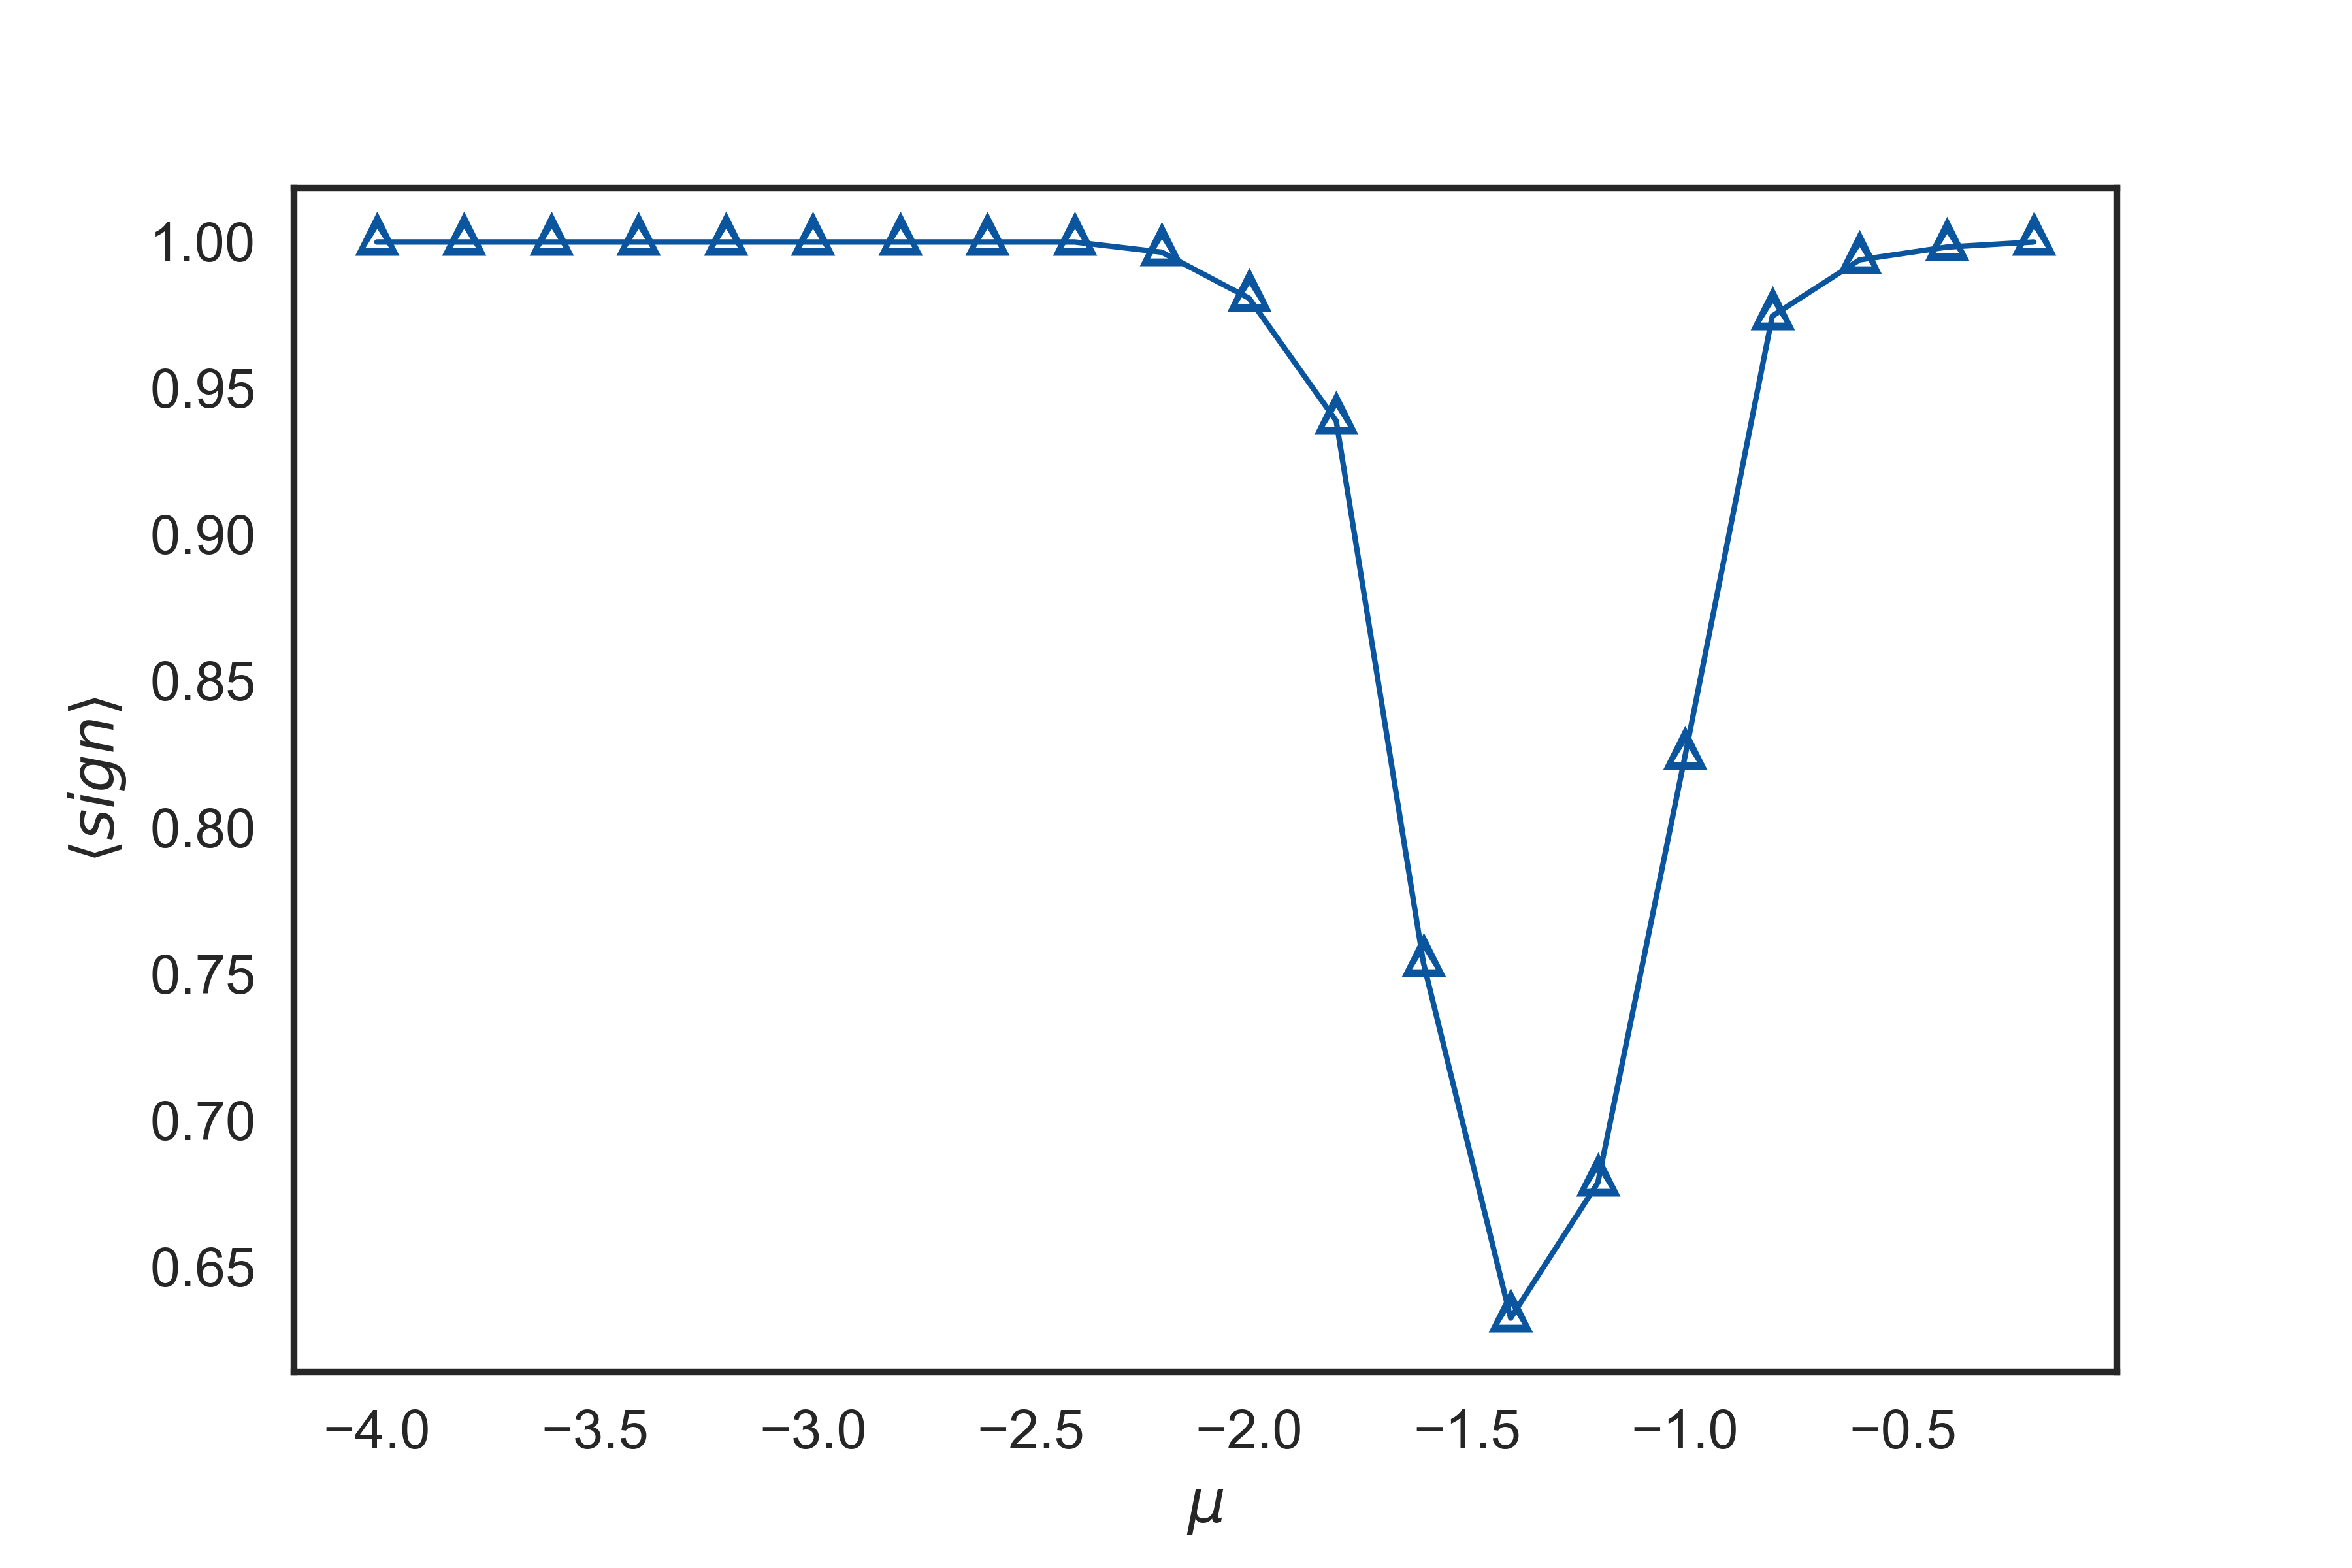
\includegraphics[scale = 0.5]{Applications/muVsSign.png}
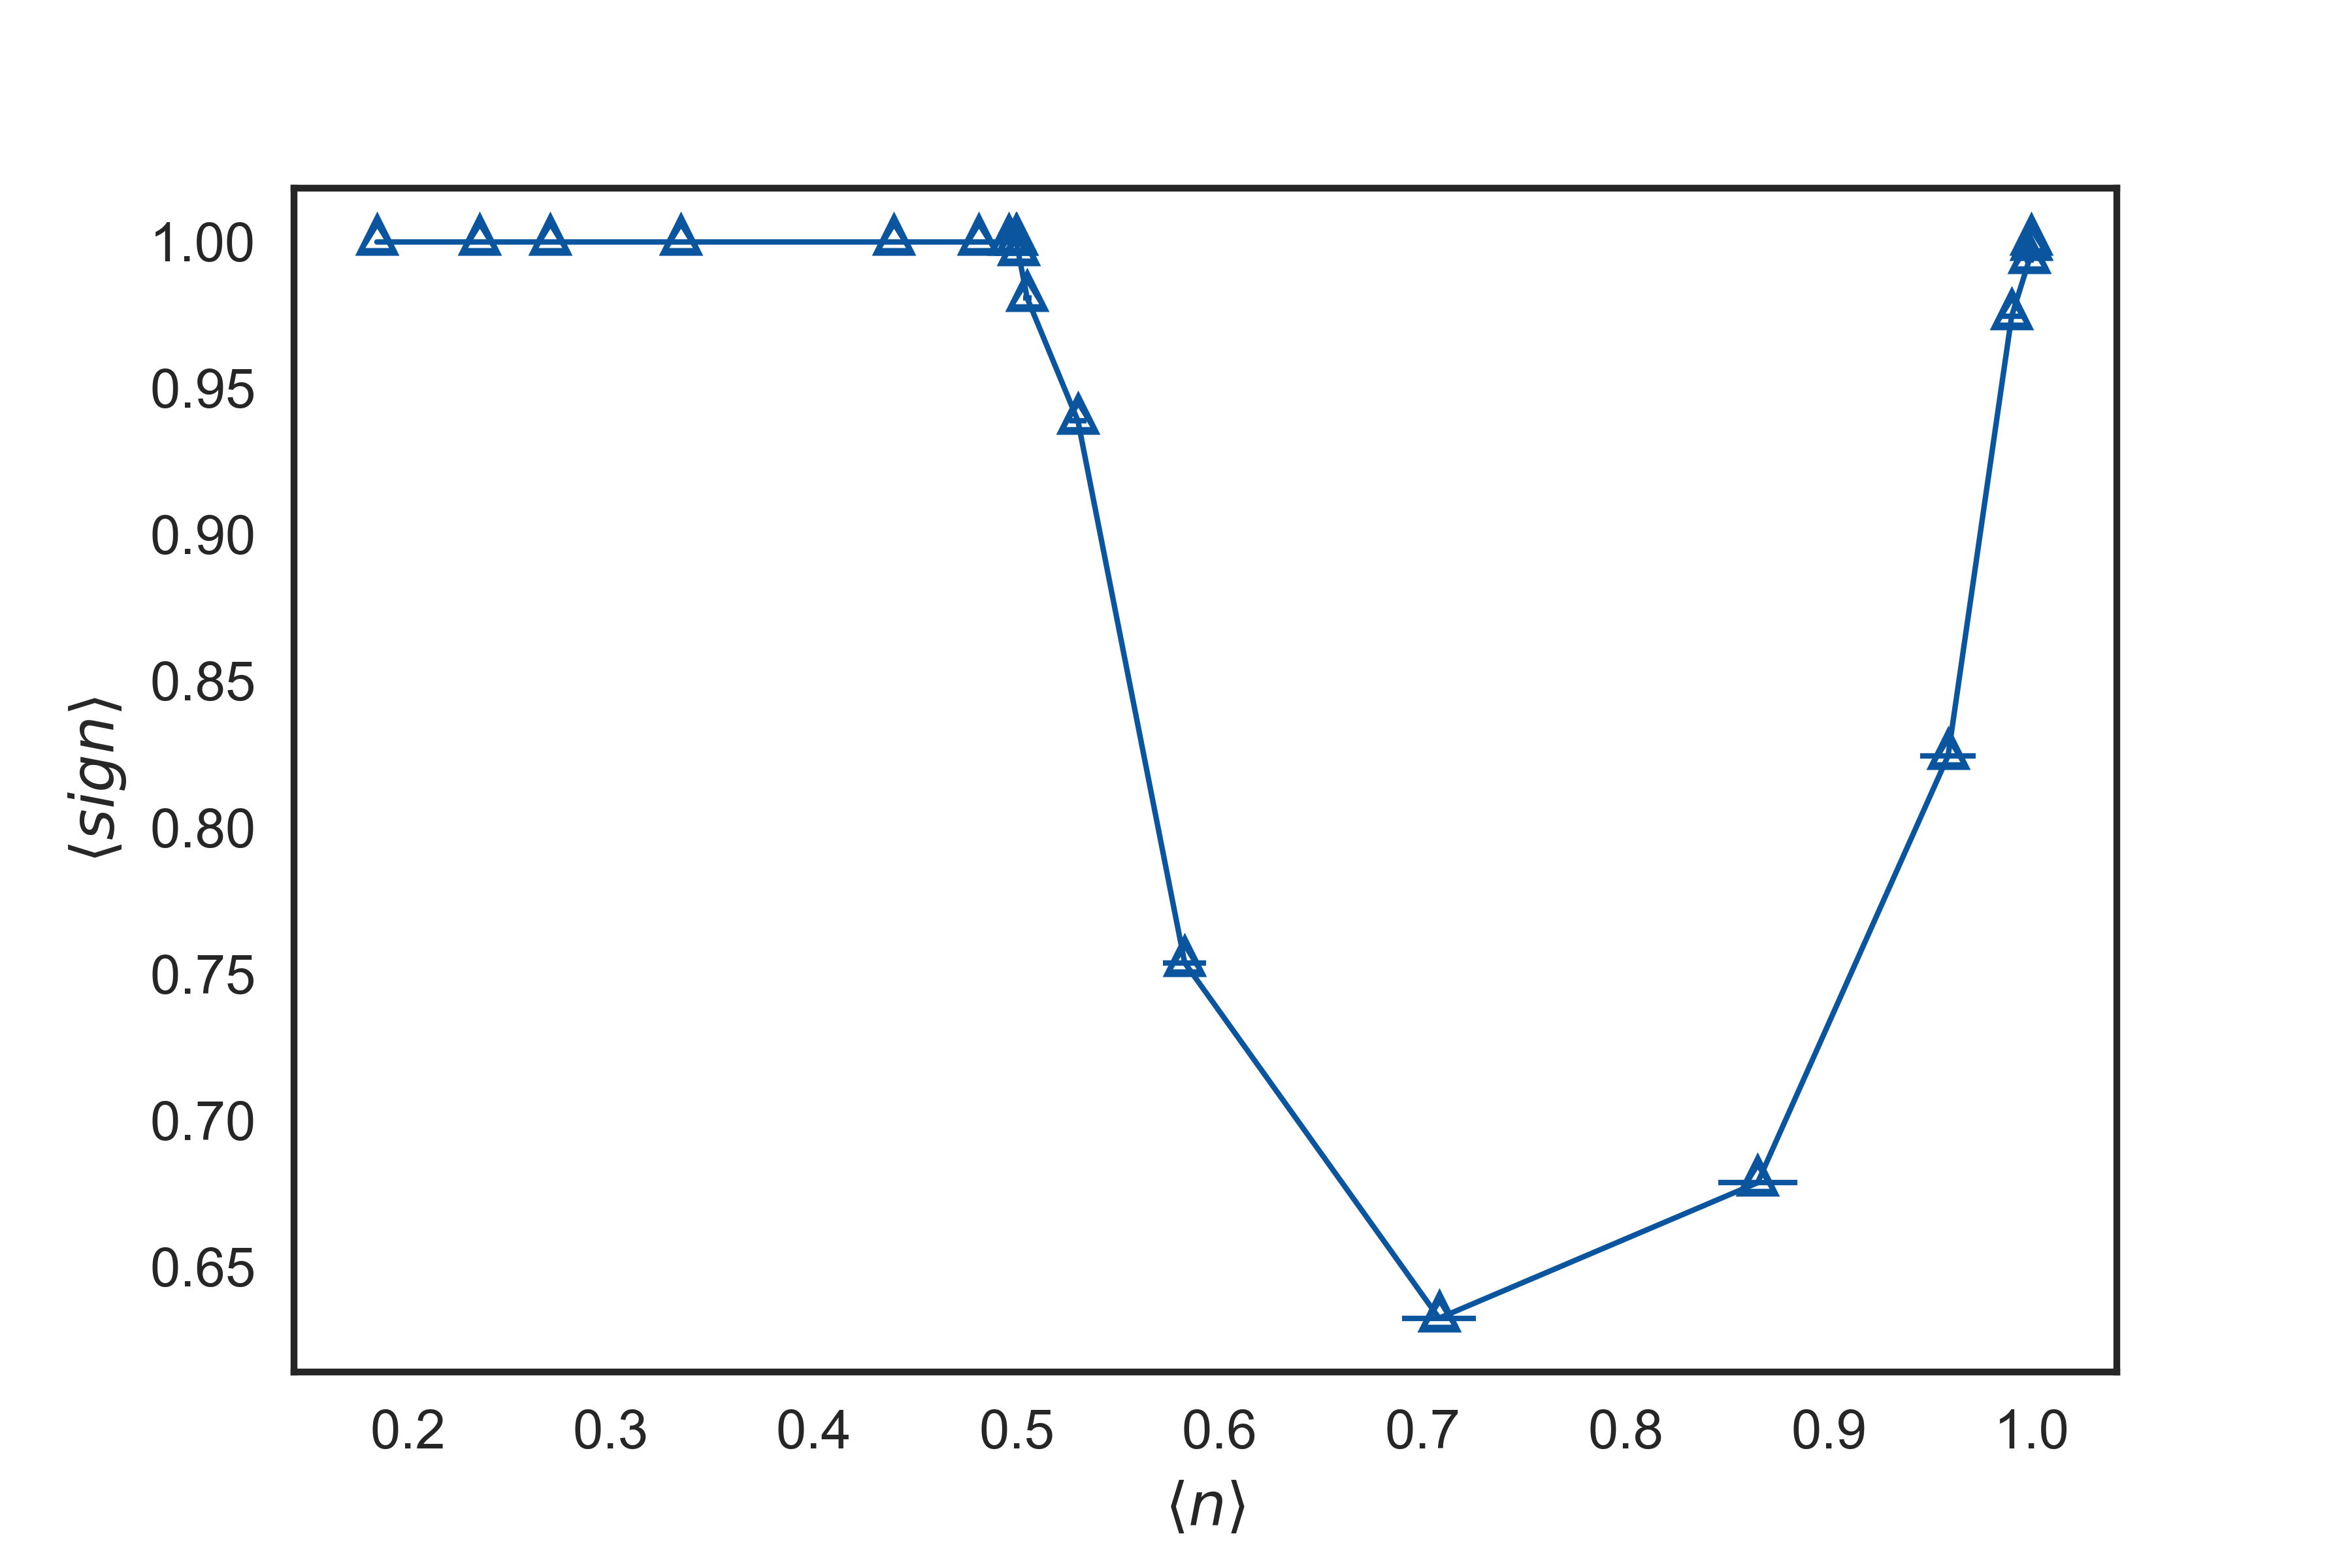
\includegraphics[scale = 0.5]{Applications/densVsSign.png}
	\caption[Average sign as a function of chemical potential/electron density for a Hubbard chain.]{Average sign as a function of chemical potential/electron density for a Hubbard chain.}
	\label{fig:signMuDens}
\end{figure}
\begin{figure}[H]
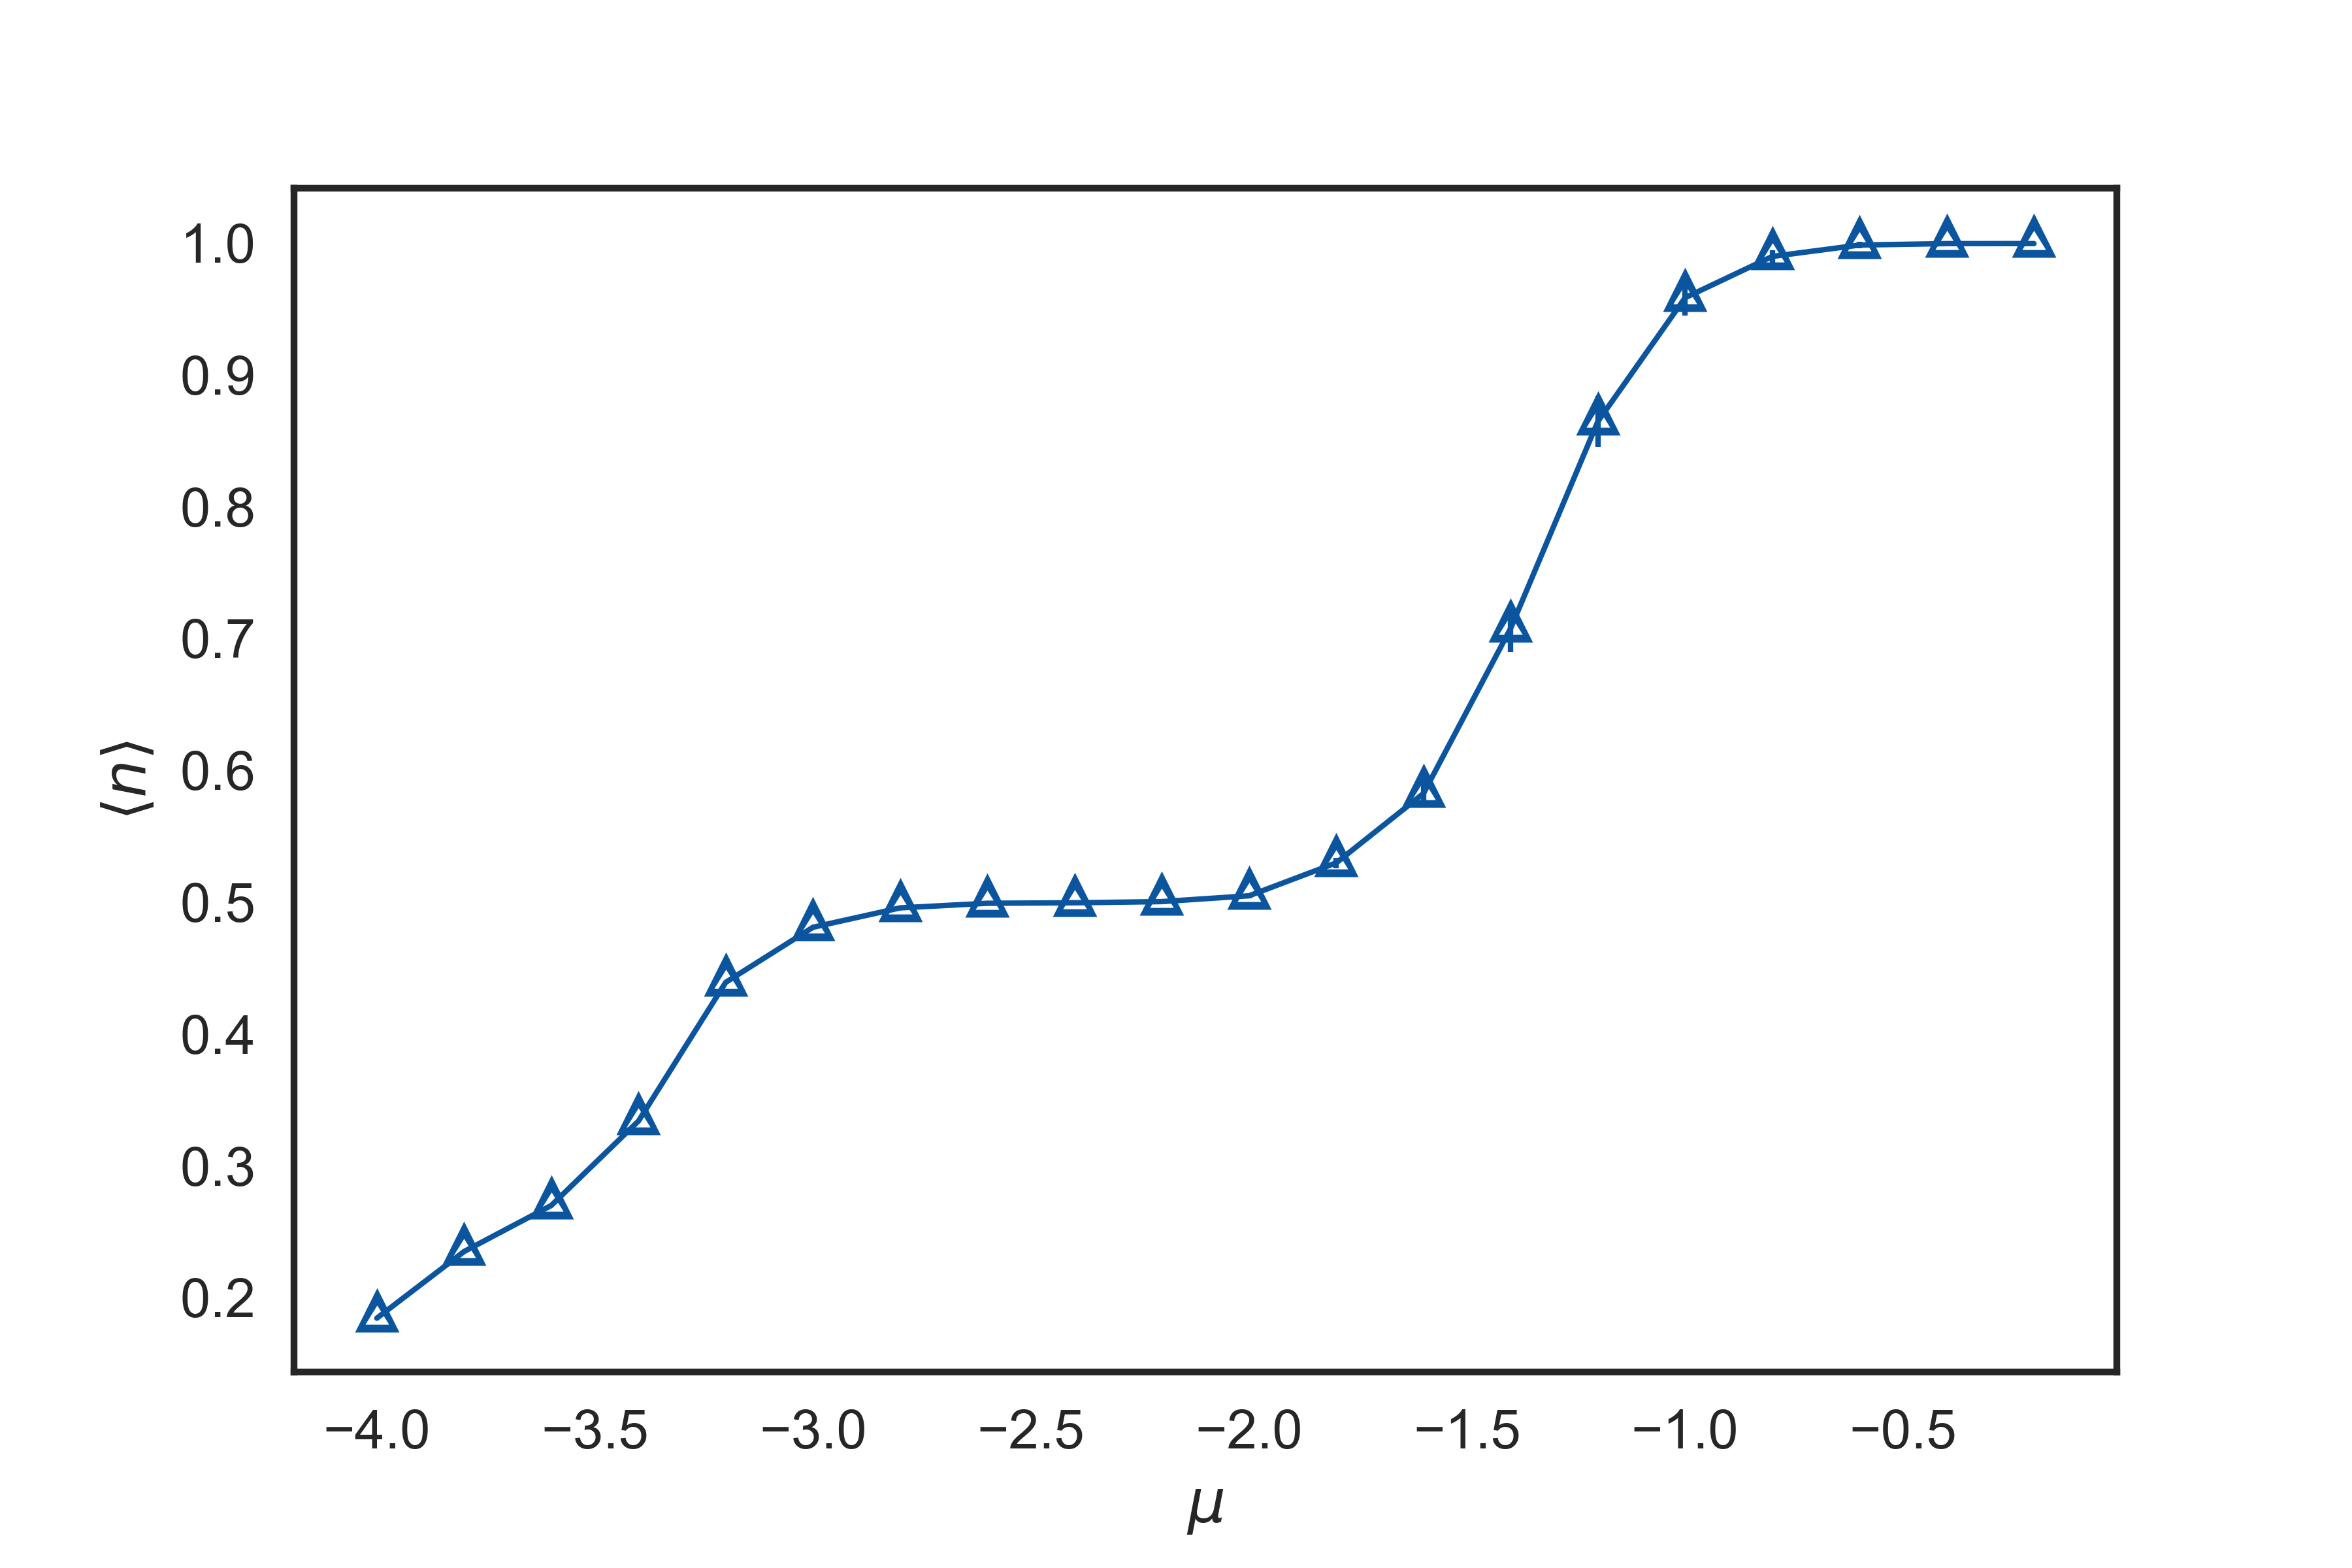
\includegraphics[scale = 0.5]{Applications/muDens.png}
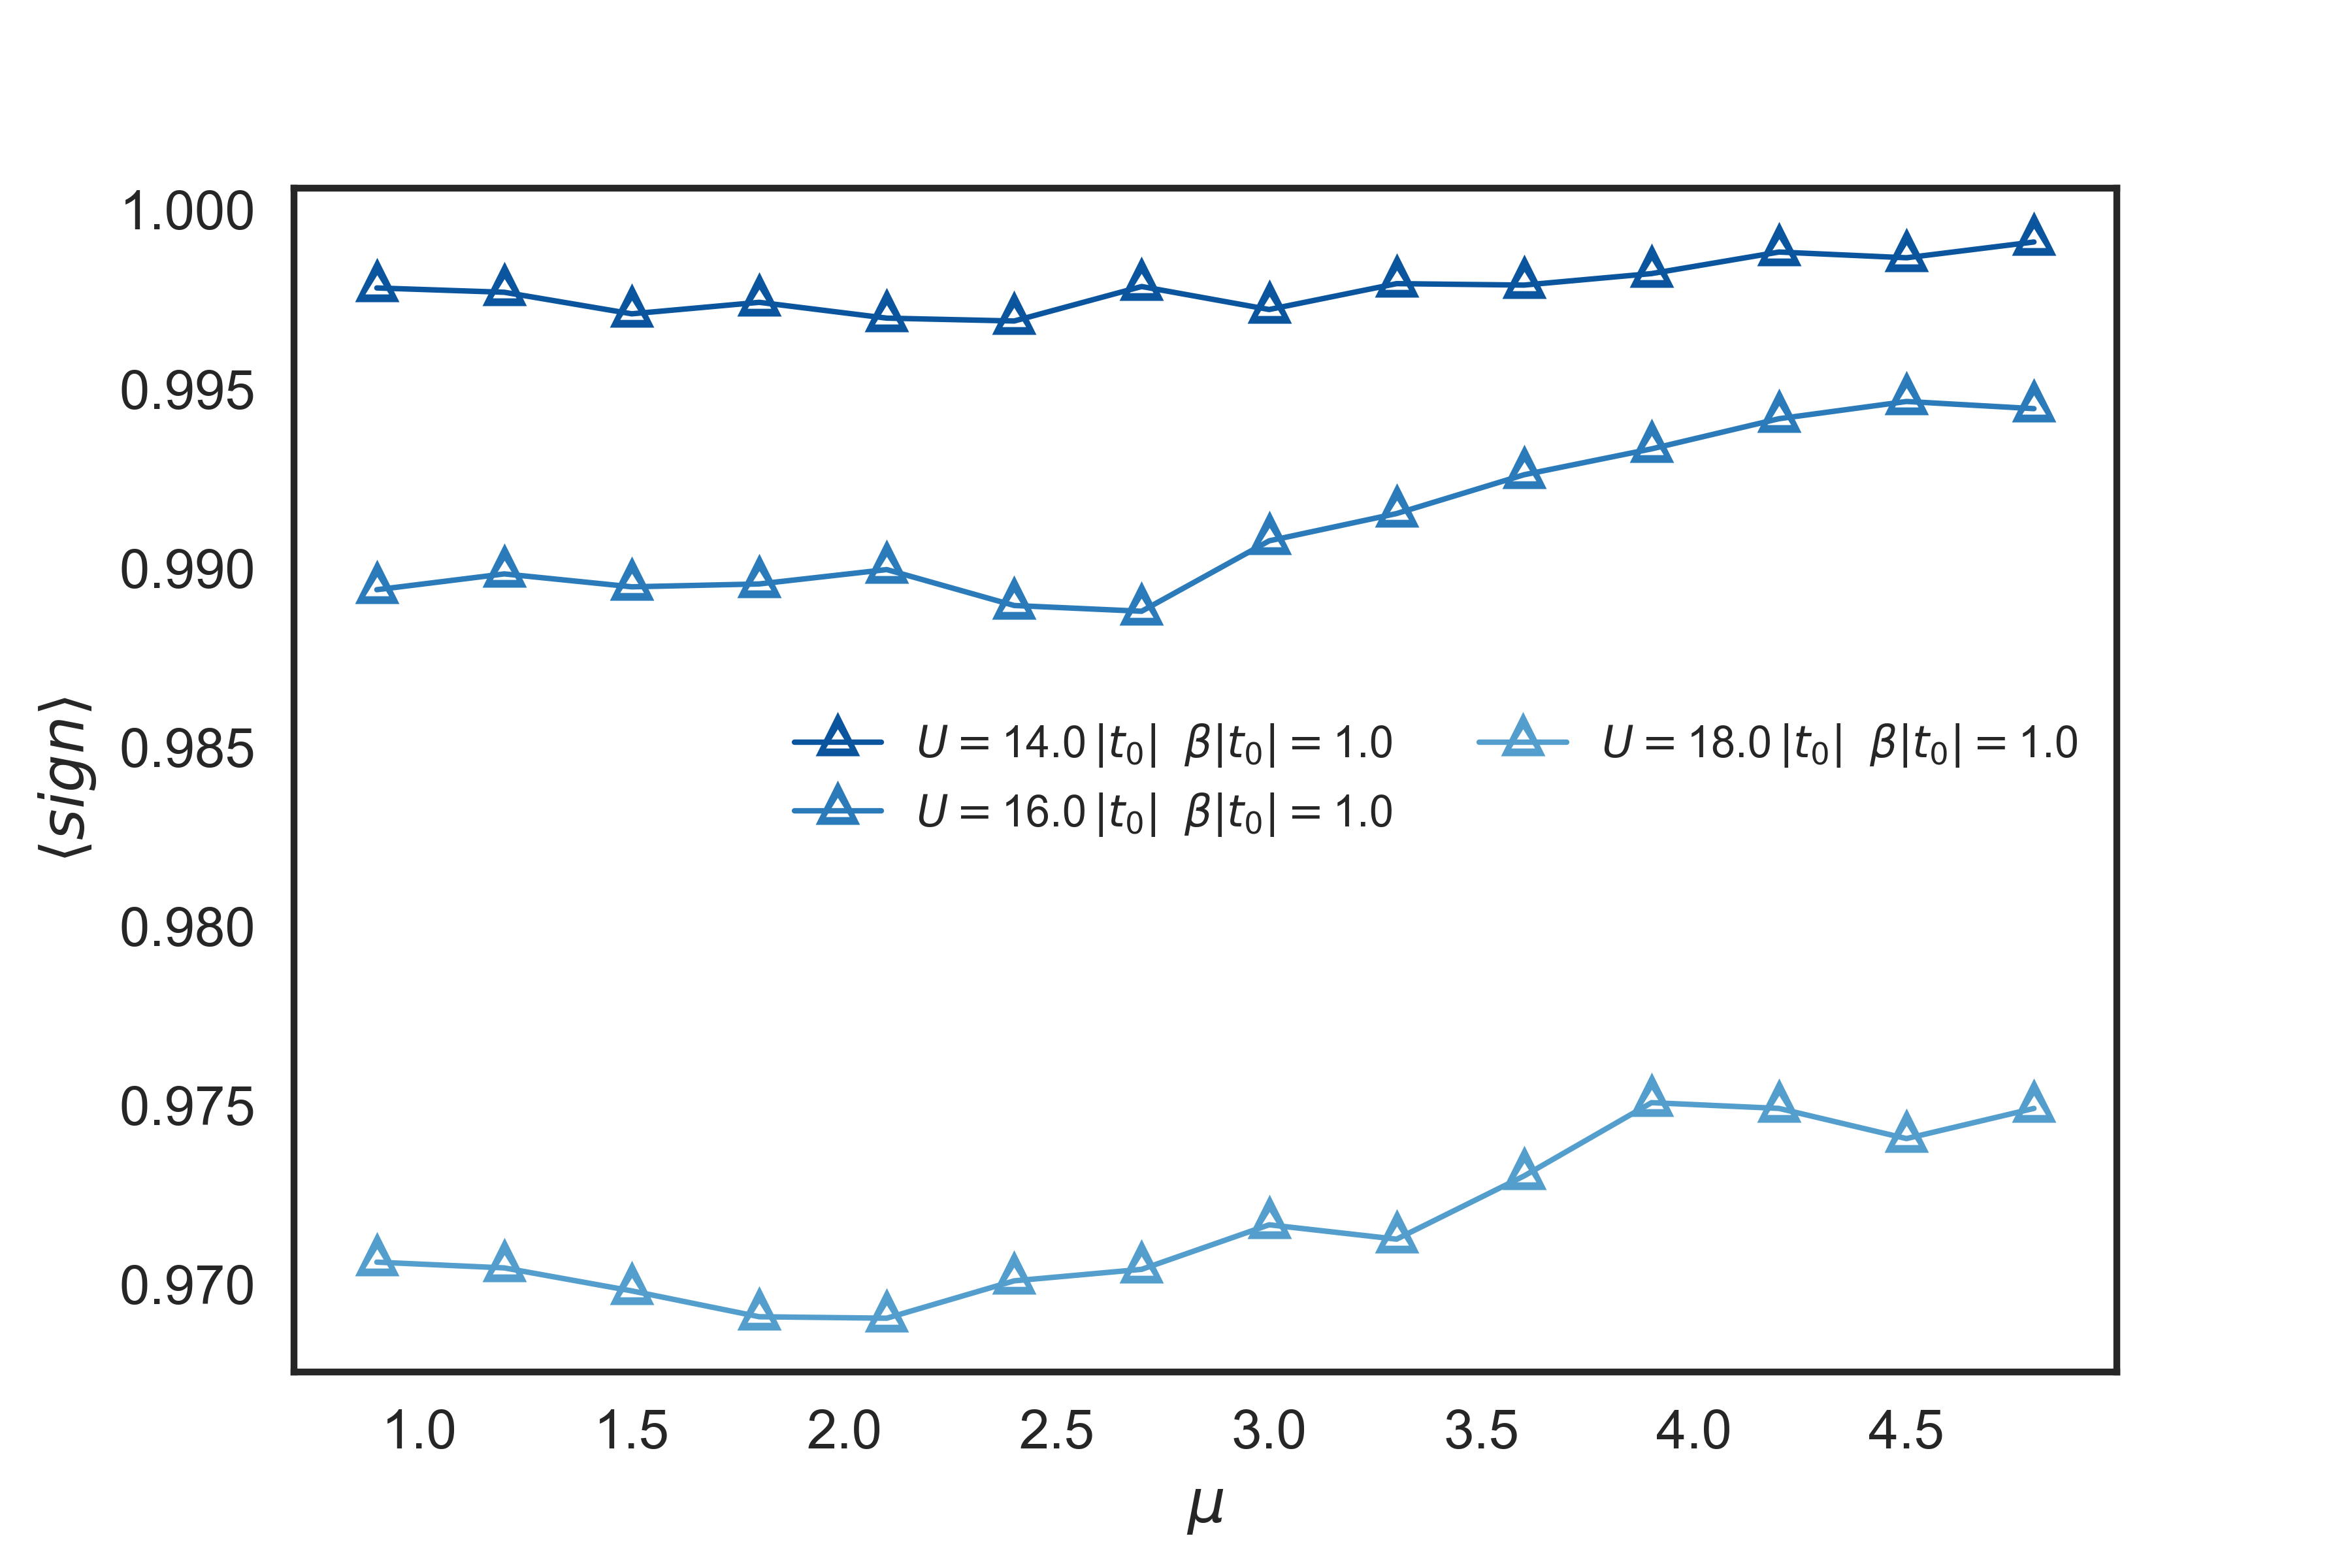
\includegraphics[scale = 0.5]{Applications/muSignTMDbeta1.png}
	\caption[Electron density as a function of chemical potential for a Hubbard chain. Average sign as a function of chemical potential for a simulation of a $9 \times 4$ TMD nanoribbon using the minimal model described in chapter 2.]{Left: Electron density as a function of chemical potential for a Hubbard chain.
	Right: Average sign as a function of chemical potential for a simulation of a $9 \times 4$ TMD nanoribbon using the minimal model described in chapter 2 at $\beta = 1$ and $U = 14, 16, 18$.
	The sign problem worsens as $U$ is increased.}
	\label{fig:muSign}
\end{figure}
\begin{figure}[H]
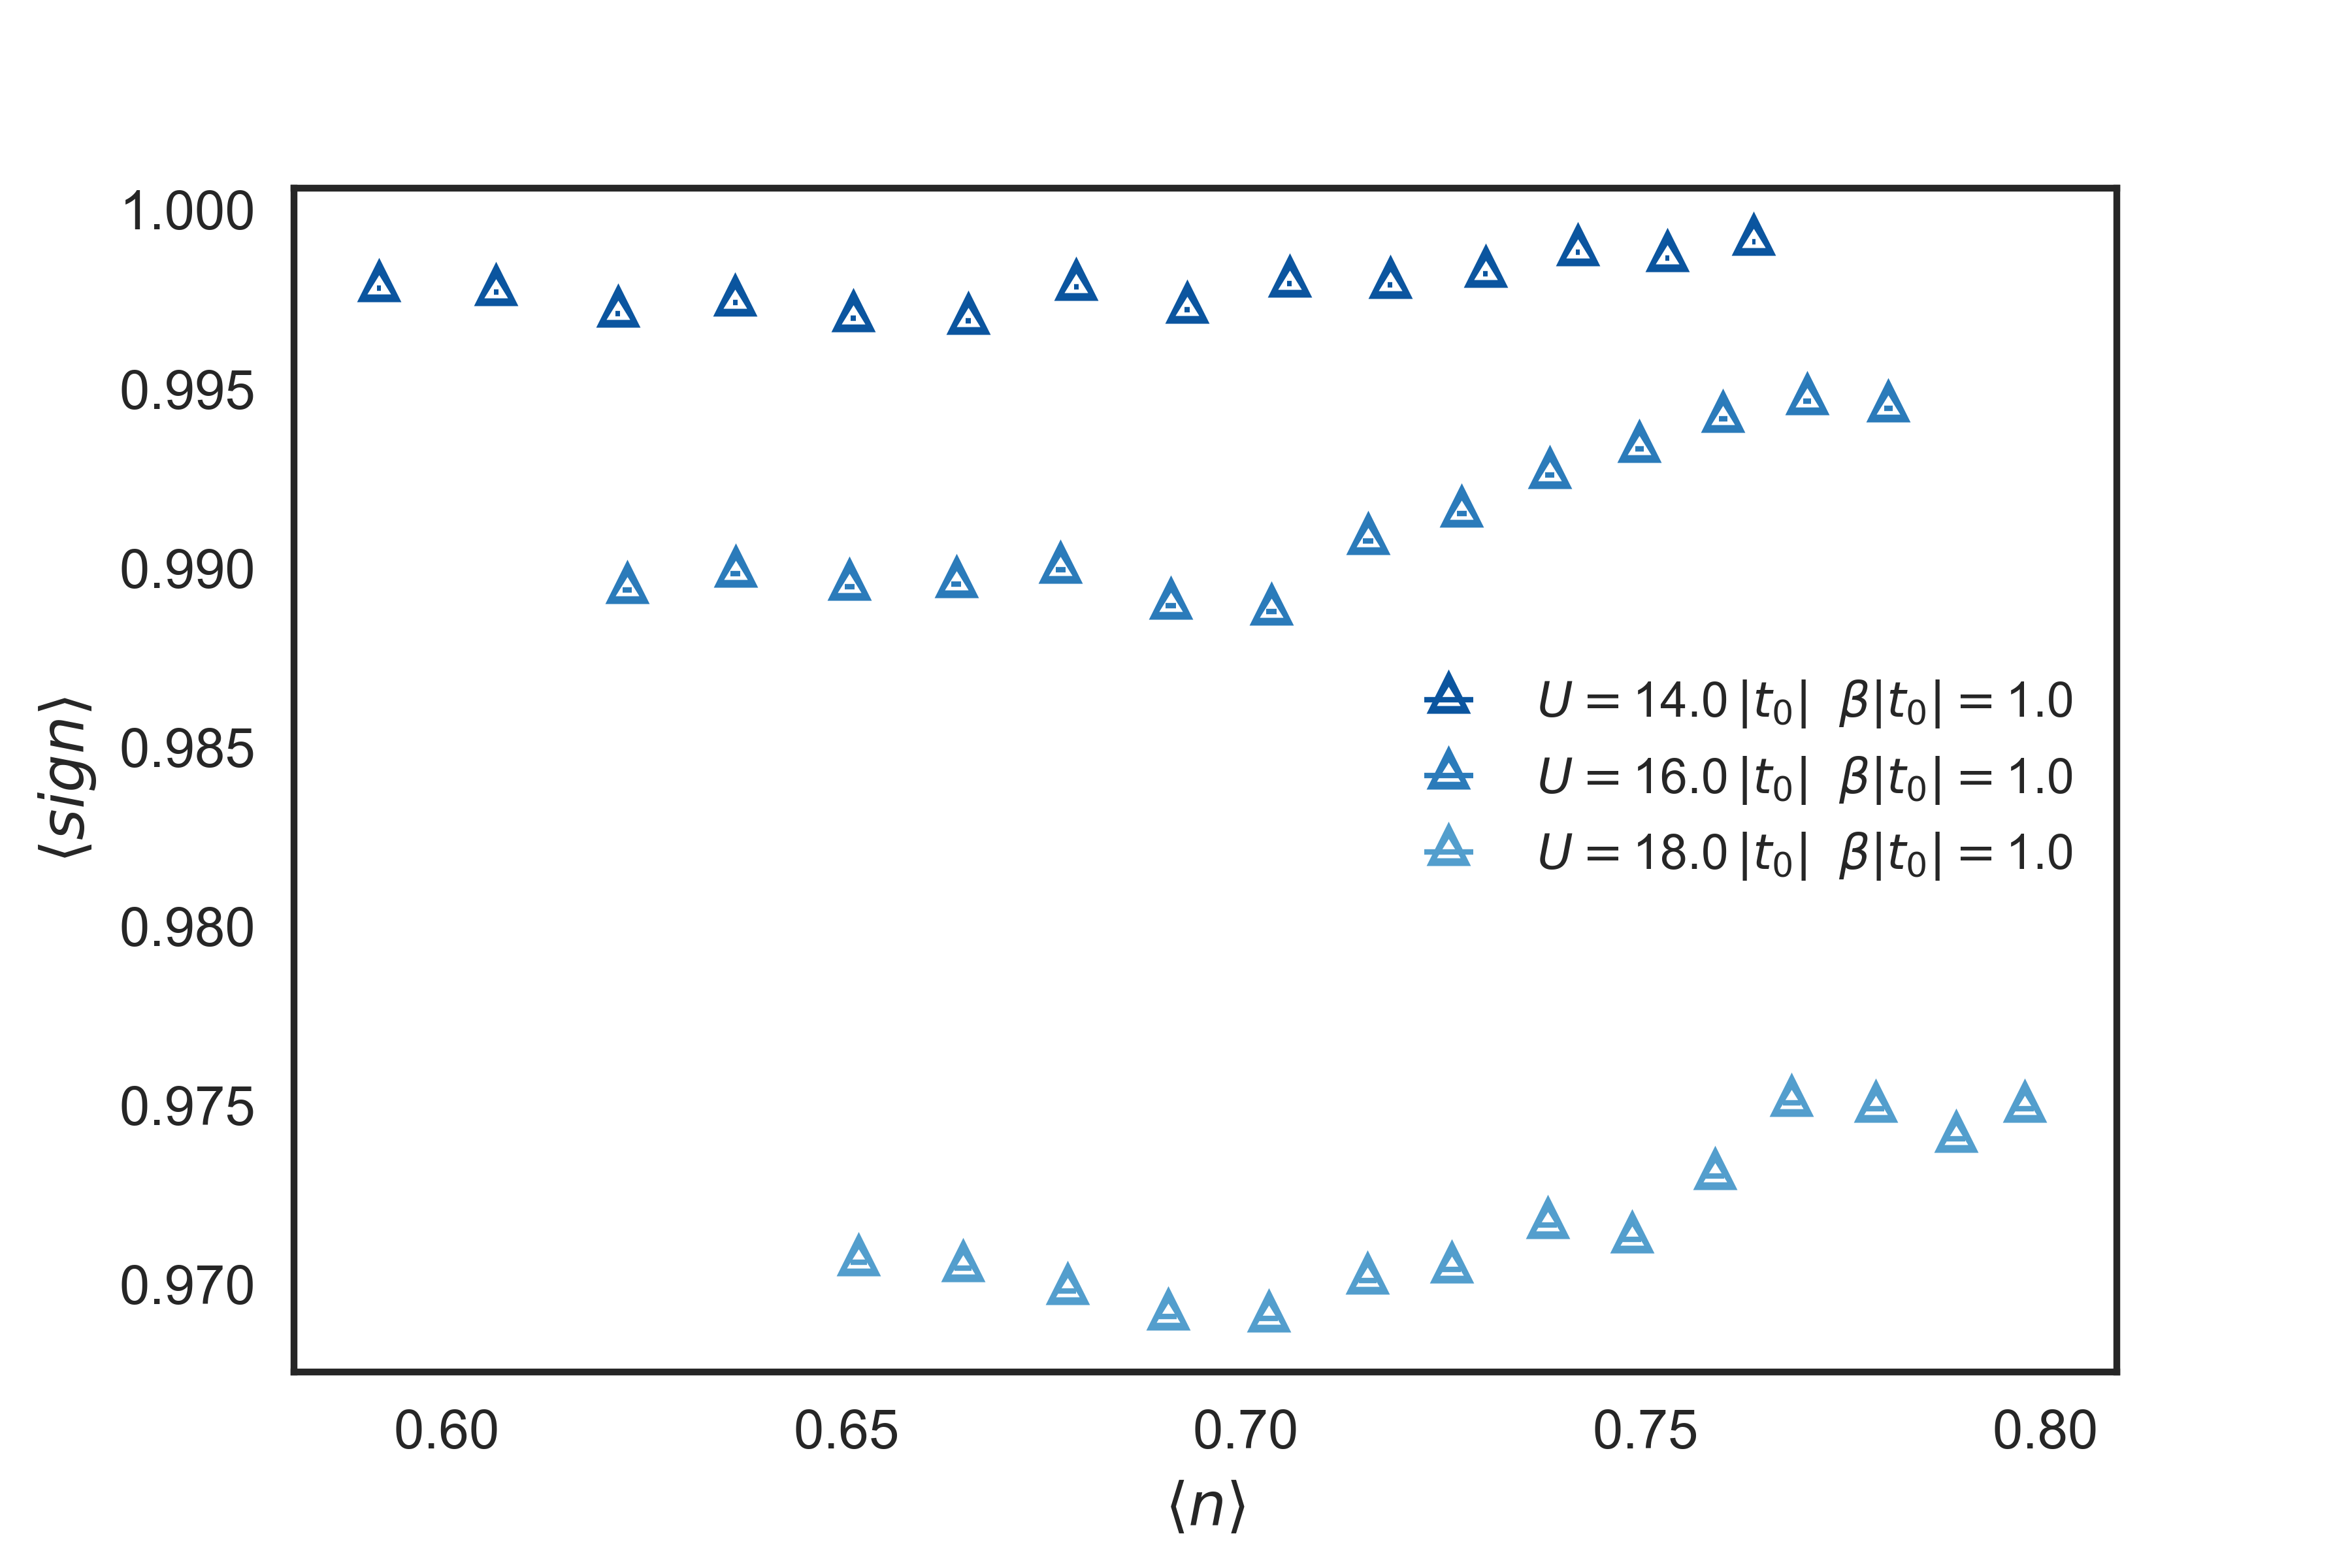
\includegraphics[scale = 0.5]{Applications/densSignTMDbeta1.png}
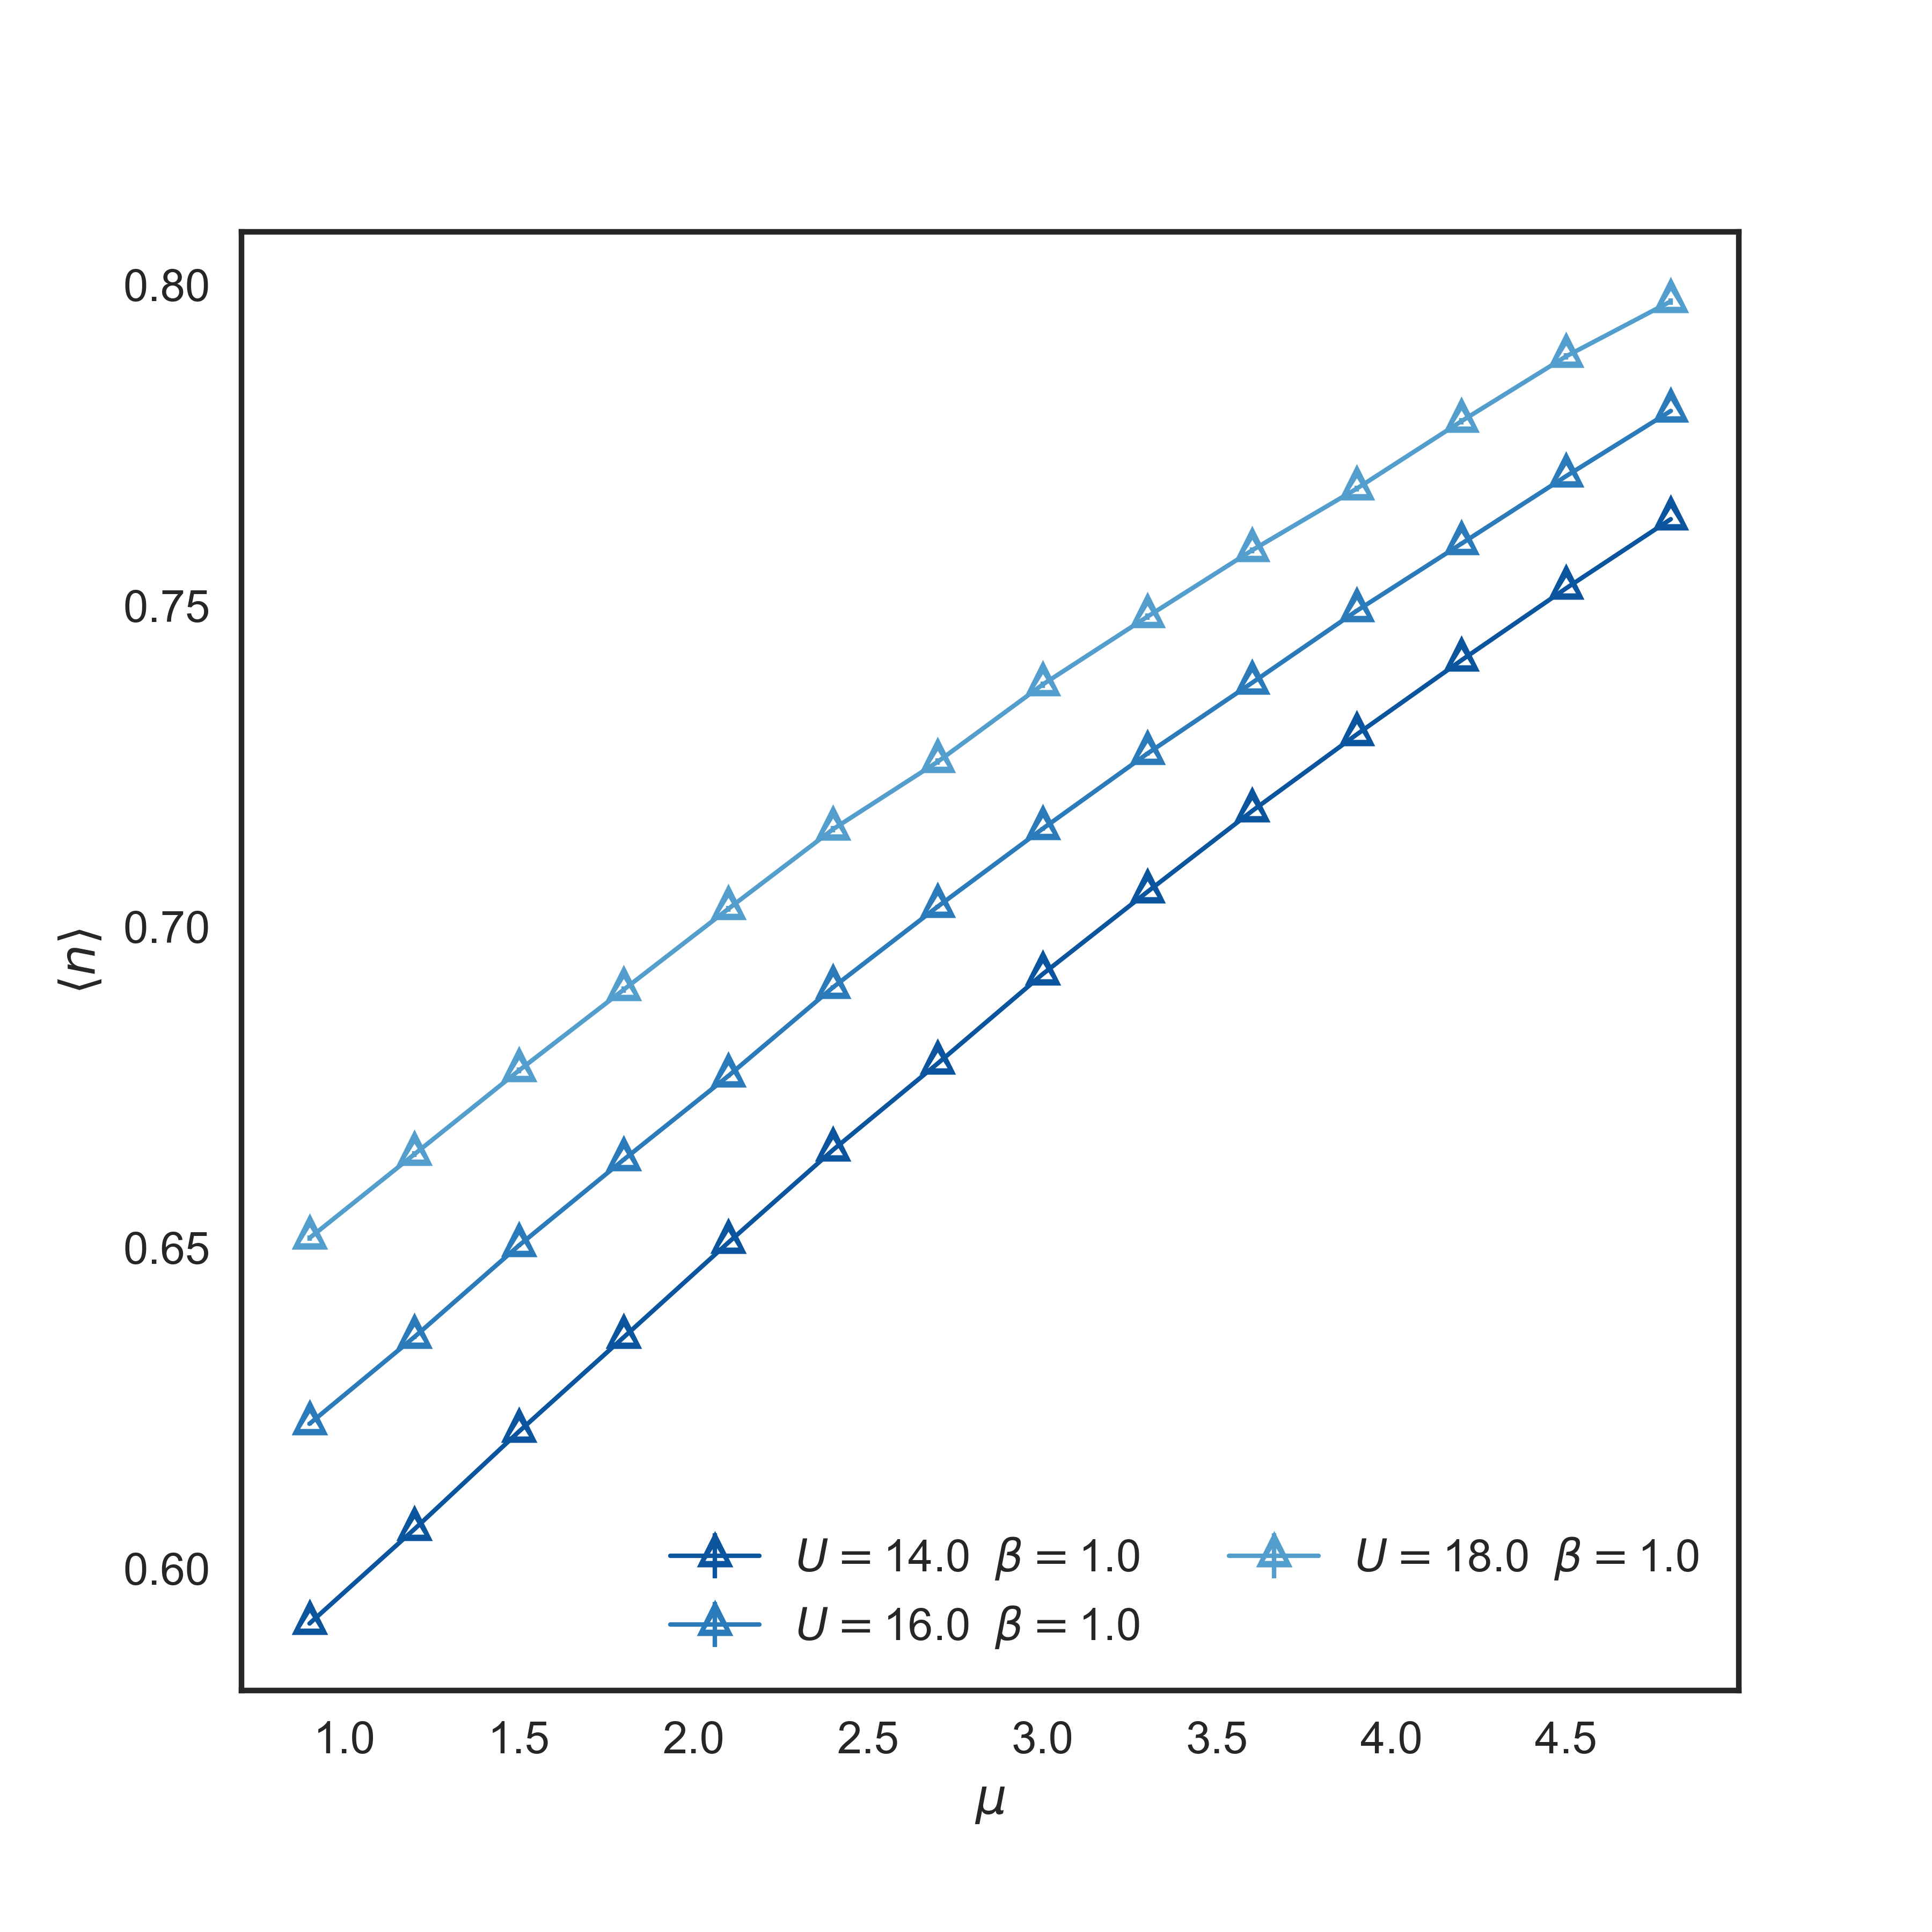
\includegraphics[scale = 0.5]{Applications/muDensTMDbeta1.png}
	\caption[Average sign as a function of electron density for the minimal Hubbard model of \acs{TMDNR}s. Electron density as a function of chemical potential.]{Left: Average sign as a function of electron density for the minimal Hubbard model of \acs{TMDNR}s. Electron density as a function of chemical potential.}
	\label{fig:densSignmuDens}
\end{figure}
\begin{figure}[H]
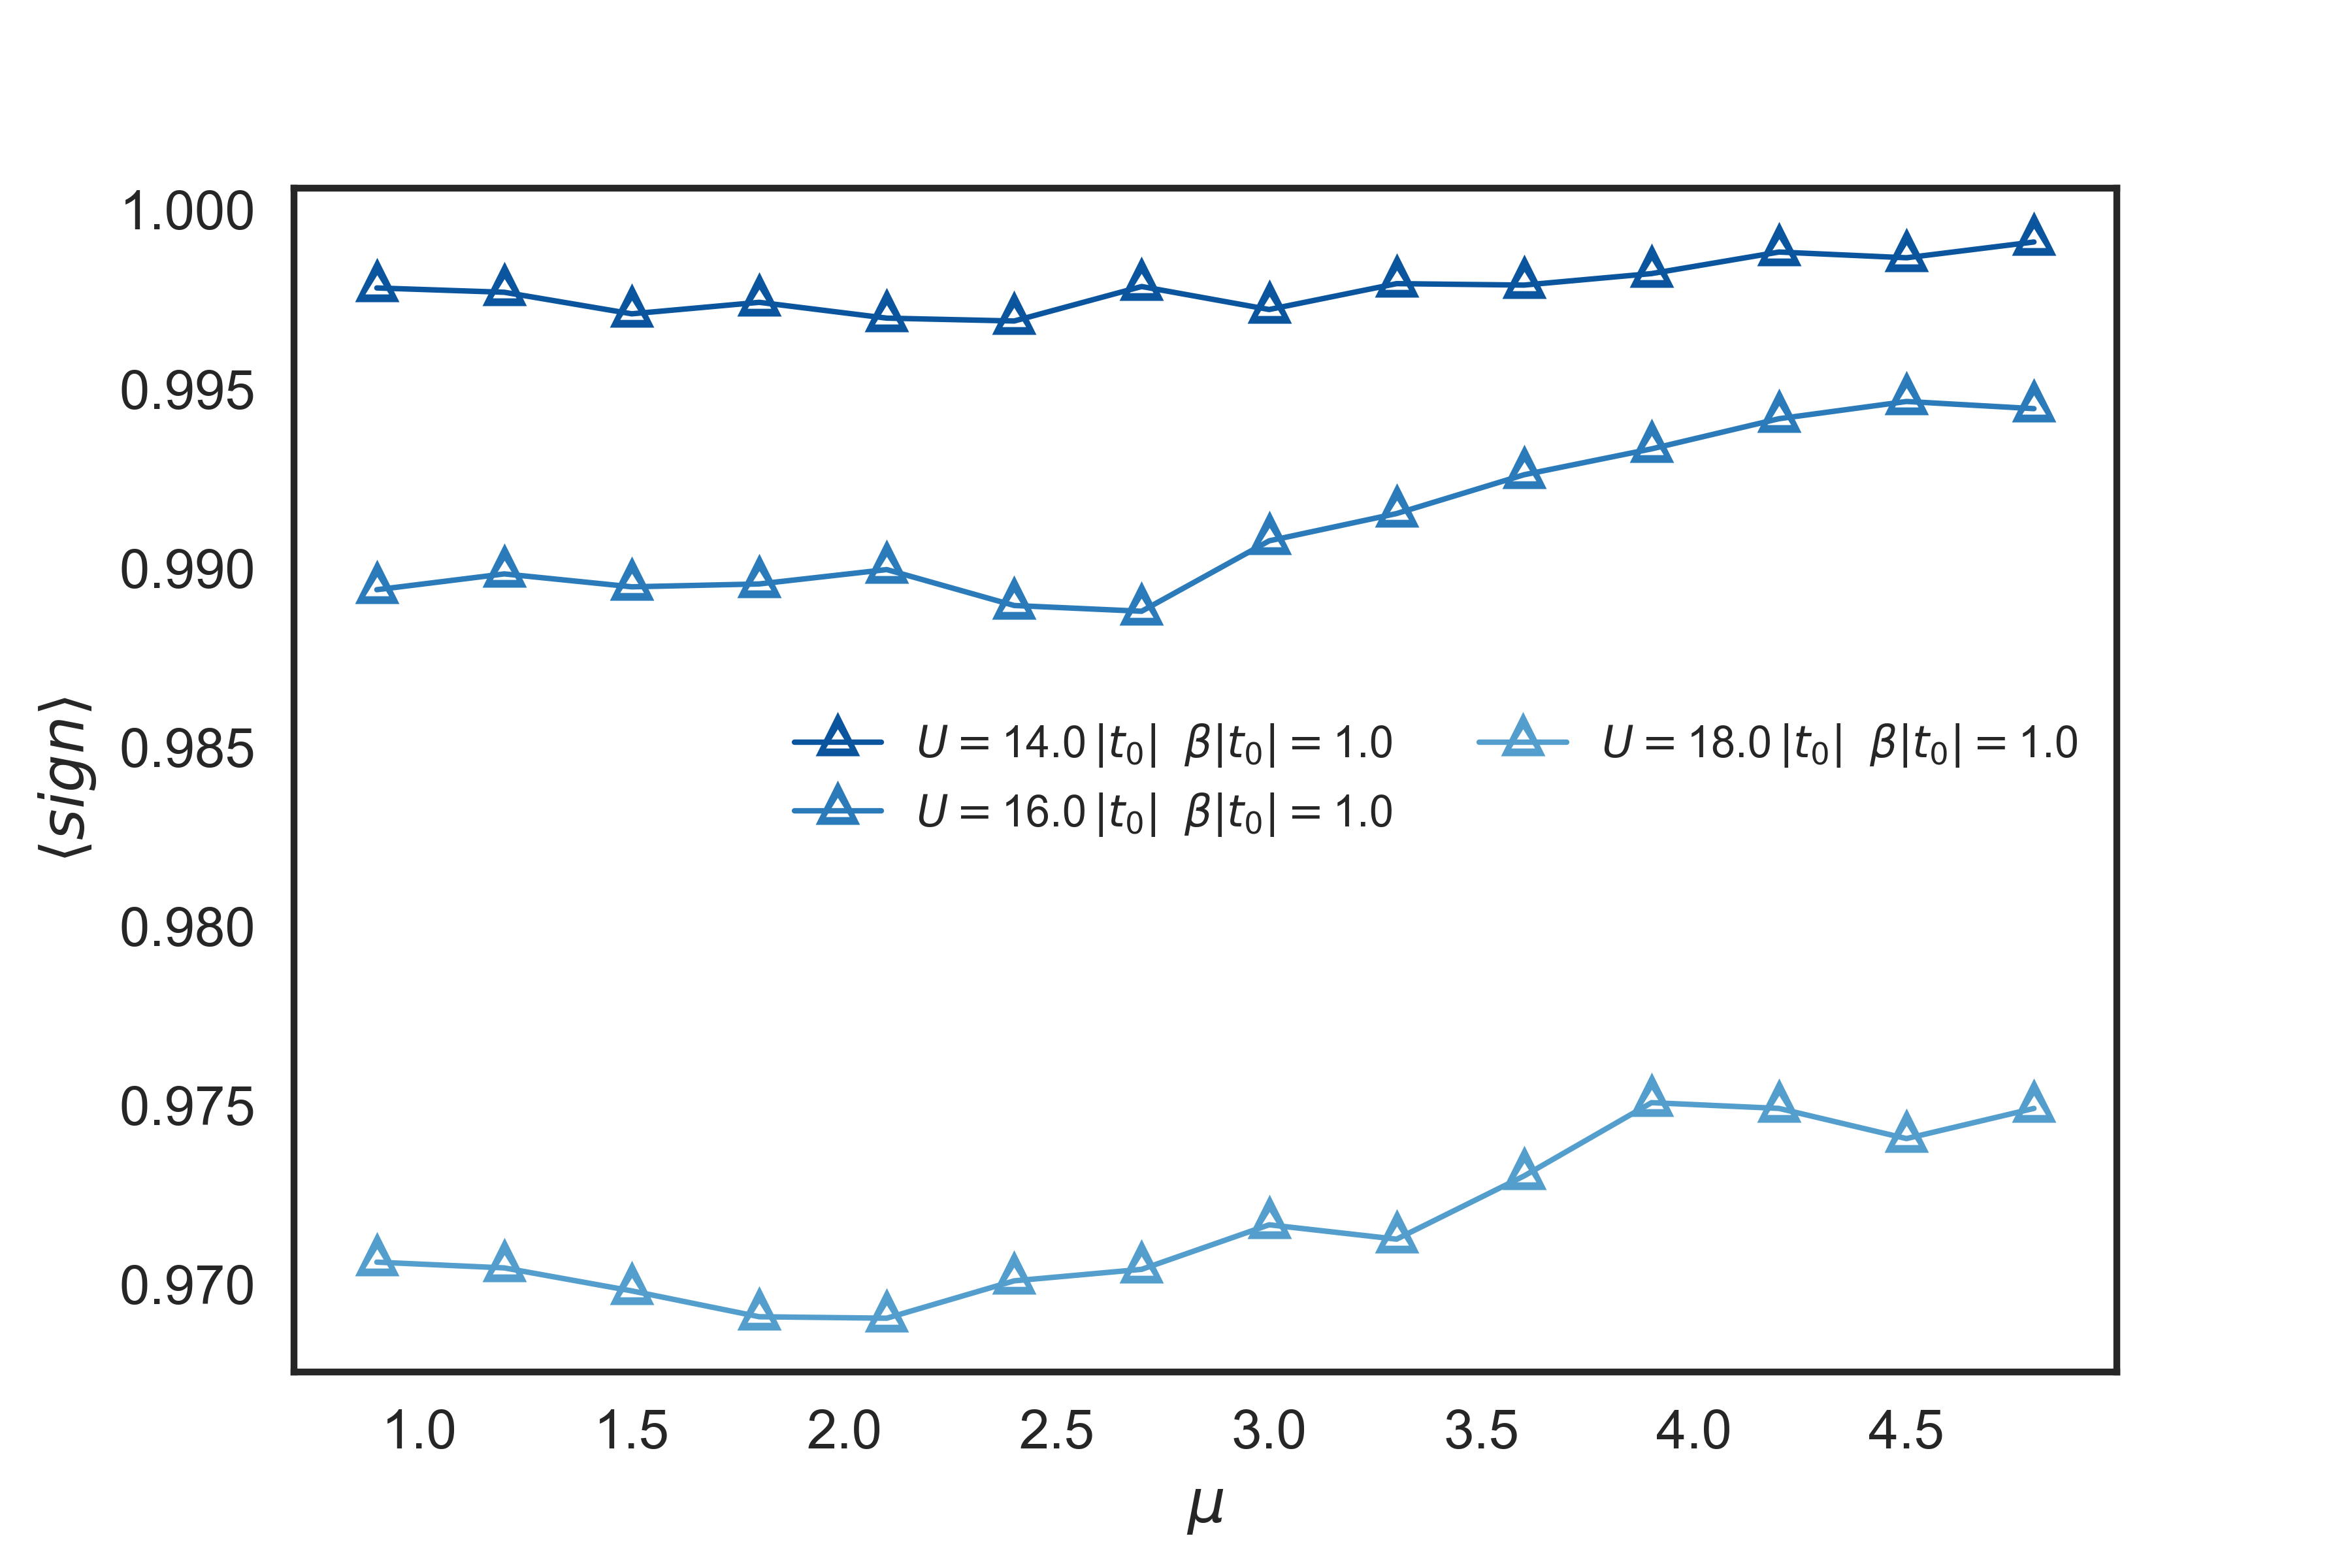
\includegraphics[scale = 0.5]{Applications/muSignTMDbeta1.png}
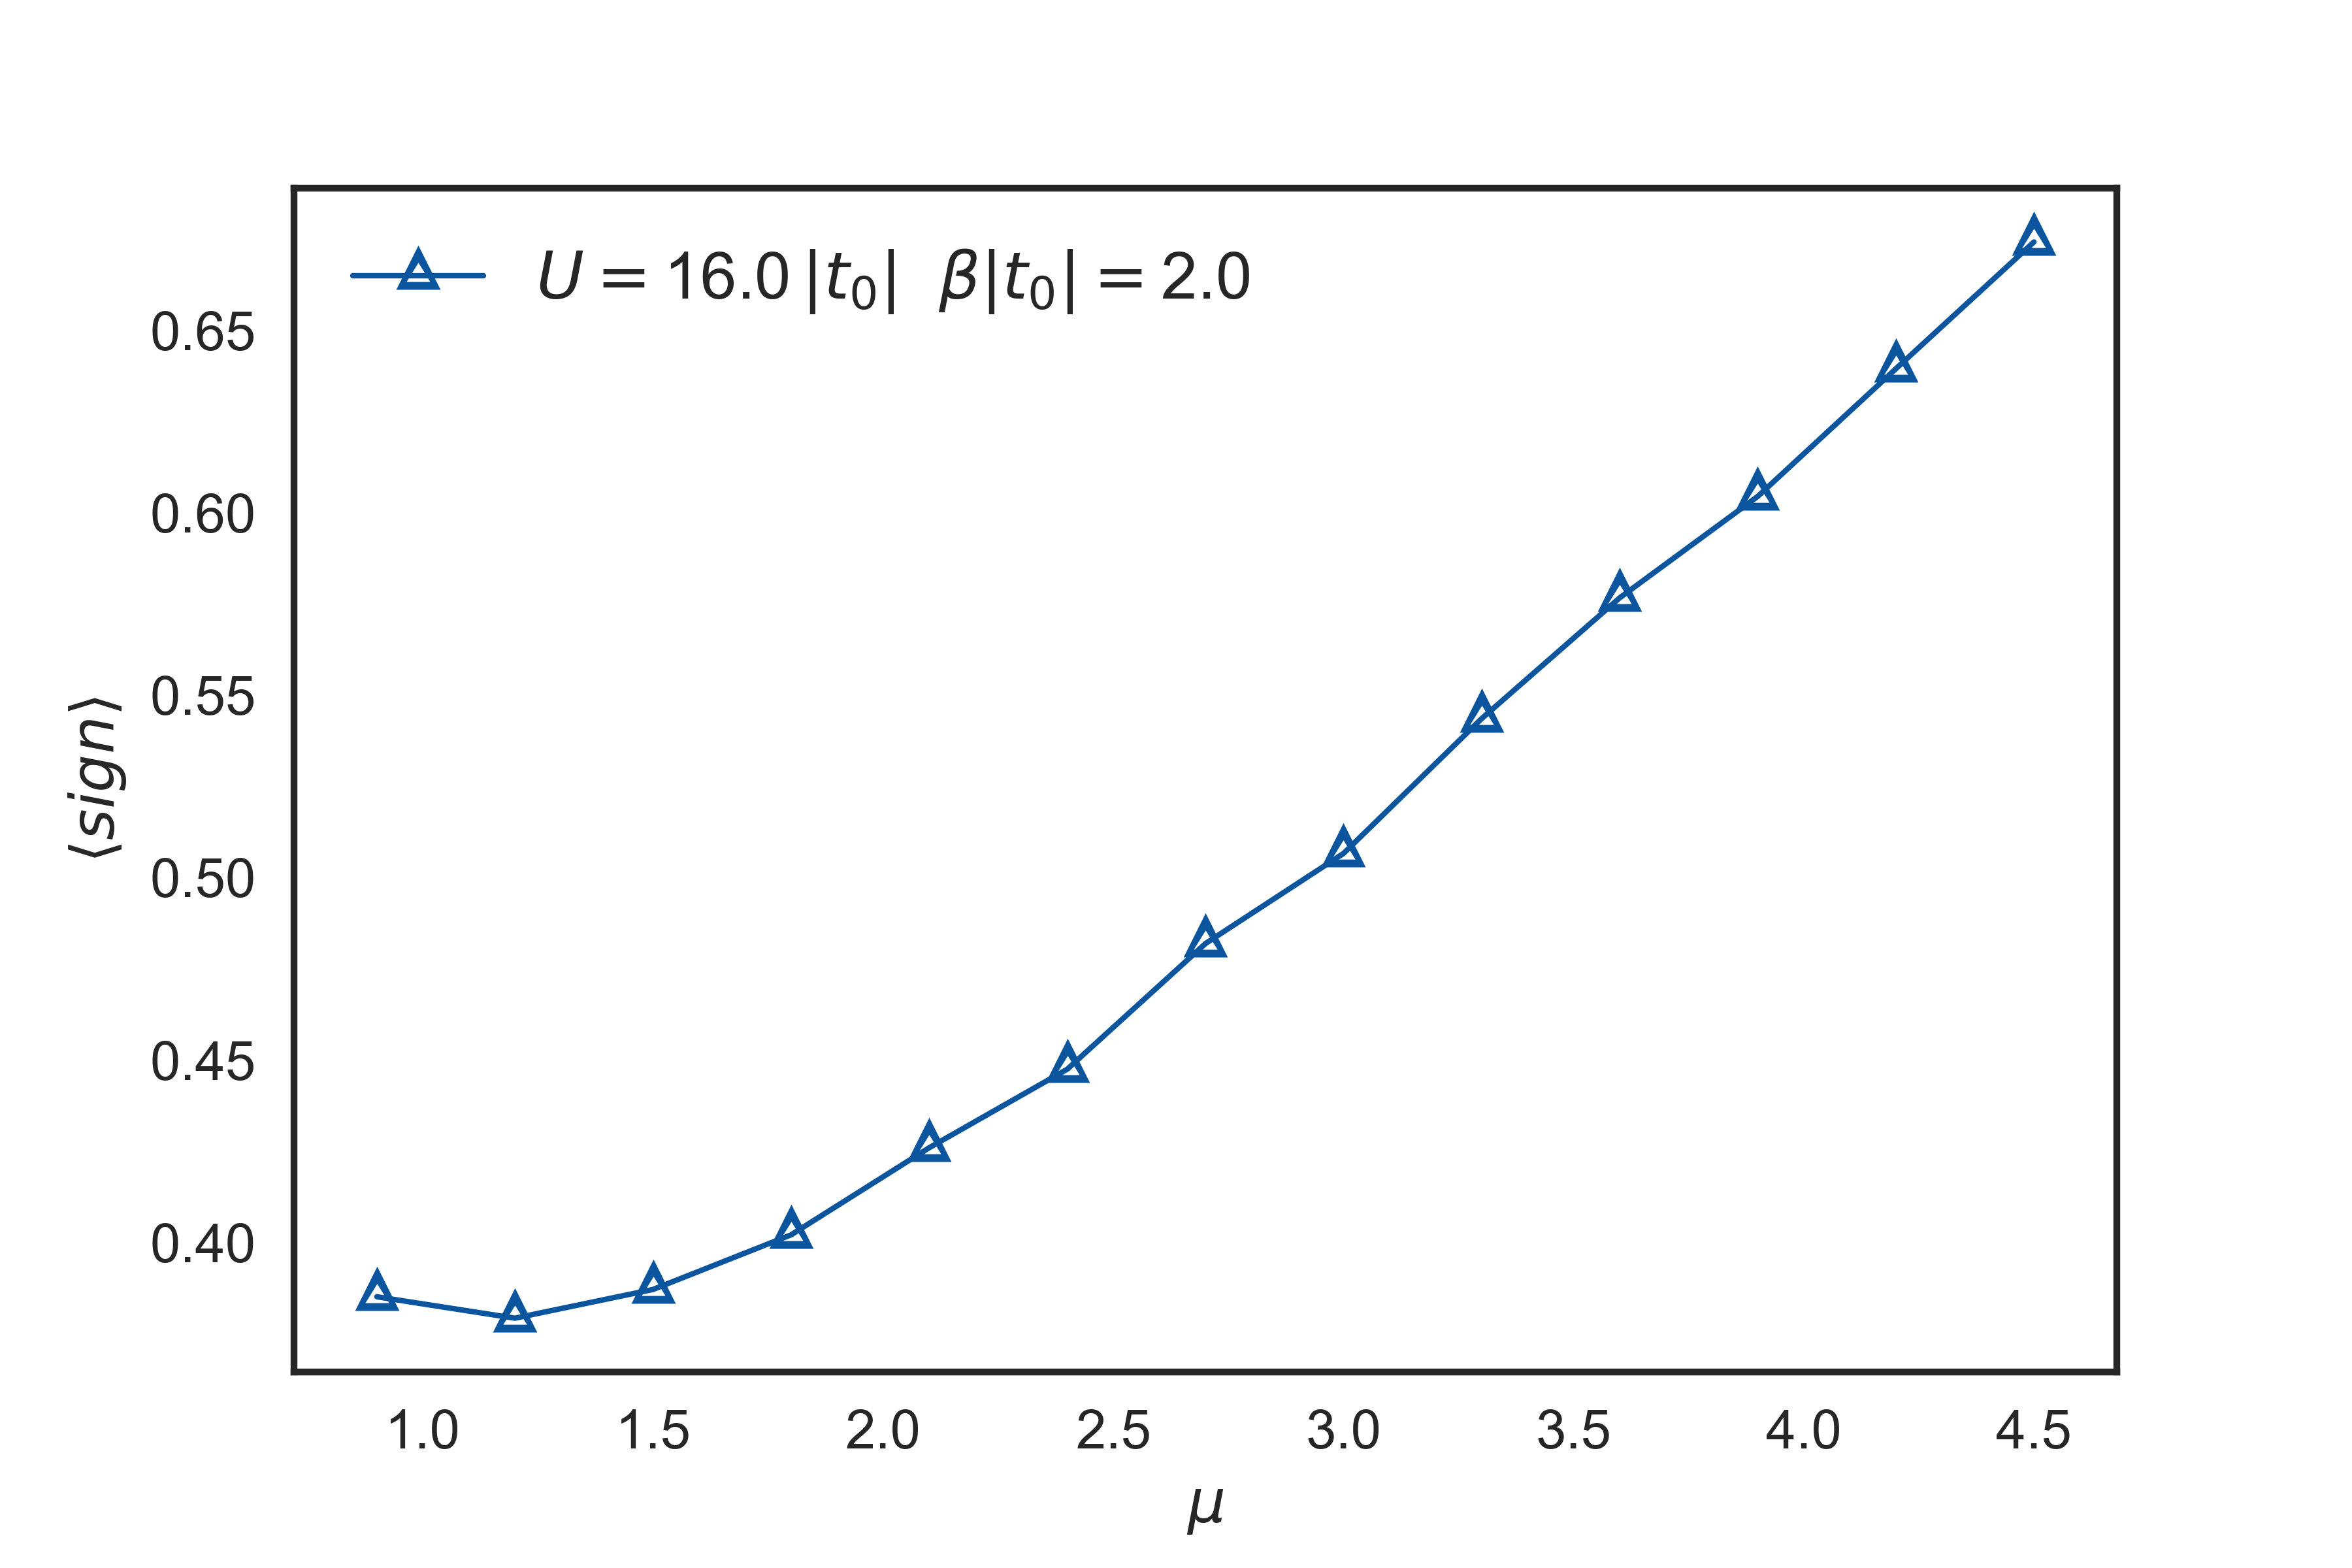
\includegraphics[scale = 0.5]{Applications/signTMDmusSignU16beta2.png}
	\caption[Average sign as a function of chemical potential for the same system, and for a system at lower temperature ($\beta = 2$), and fixed on-site/orbital interaction $U = 16$.]{Average sign as a function of chemical potential for the same system (left), and for a system at lower temperature ($\beta = 2$), and fixed on-site/orbital interaction $U = 16$ (right).}
	\label{fig:muDensU16signDens}
\end{figure}
\begin{figure}[H]
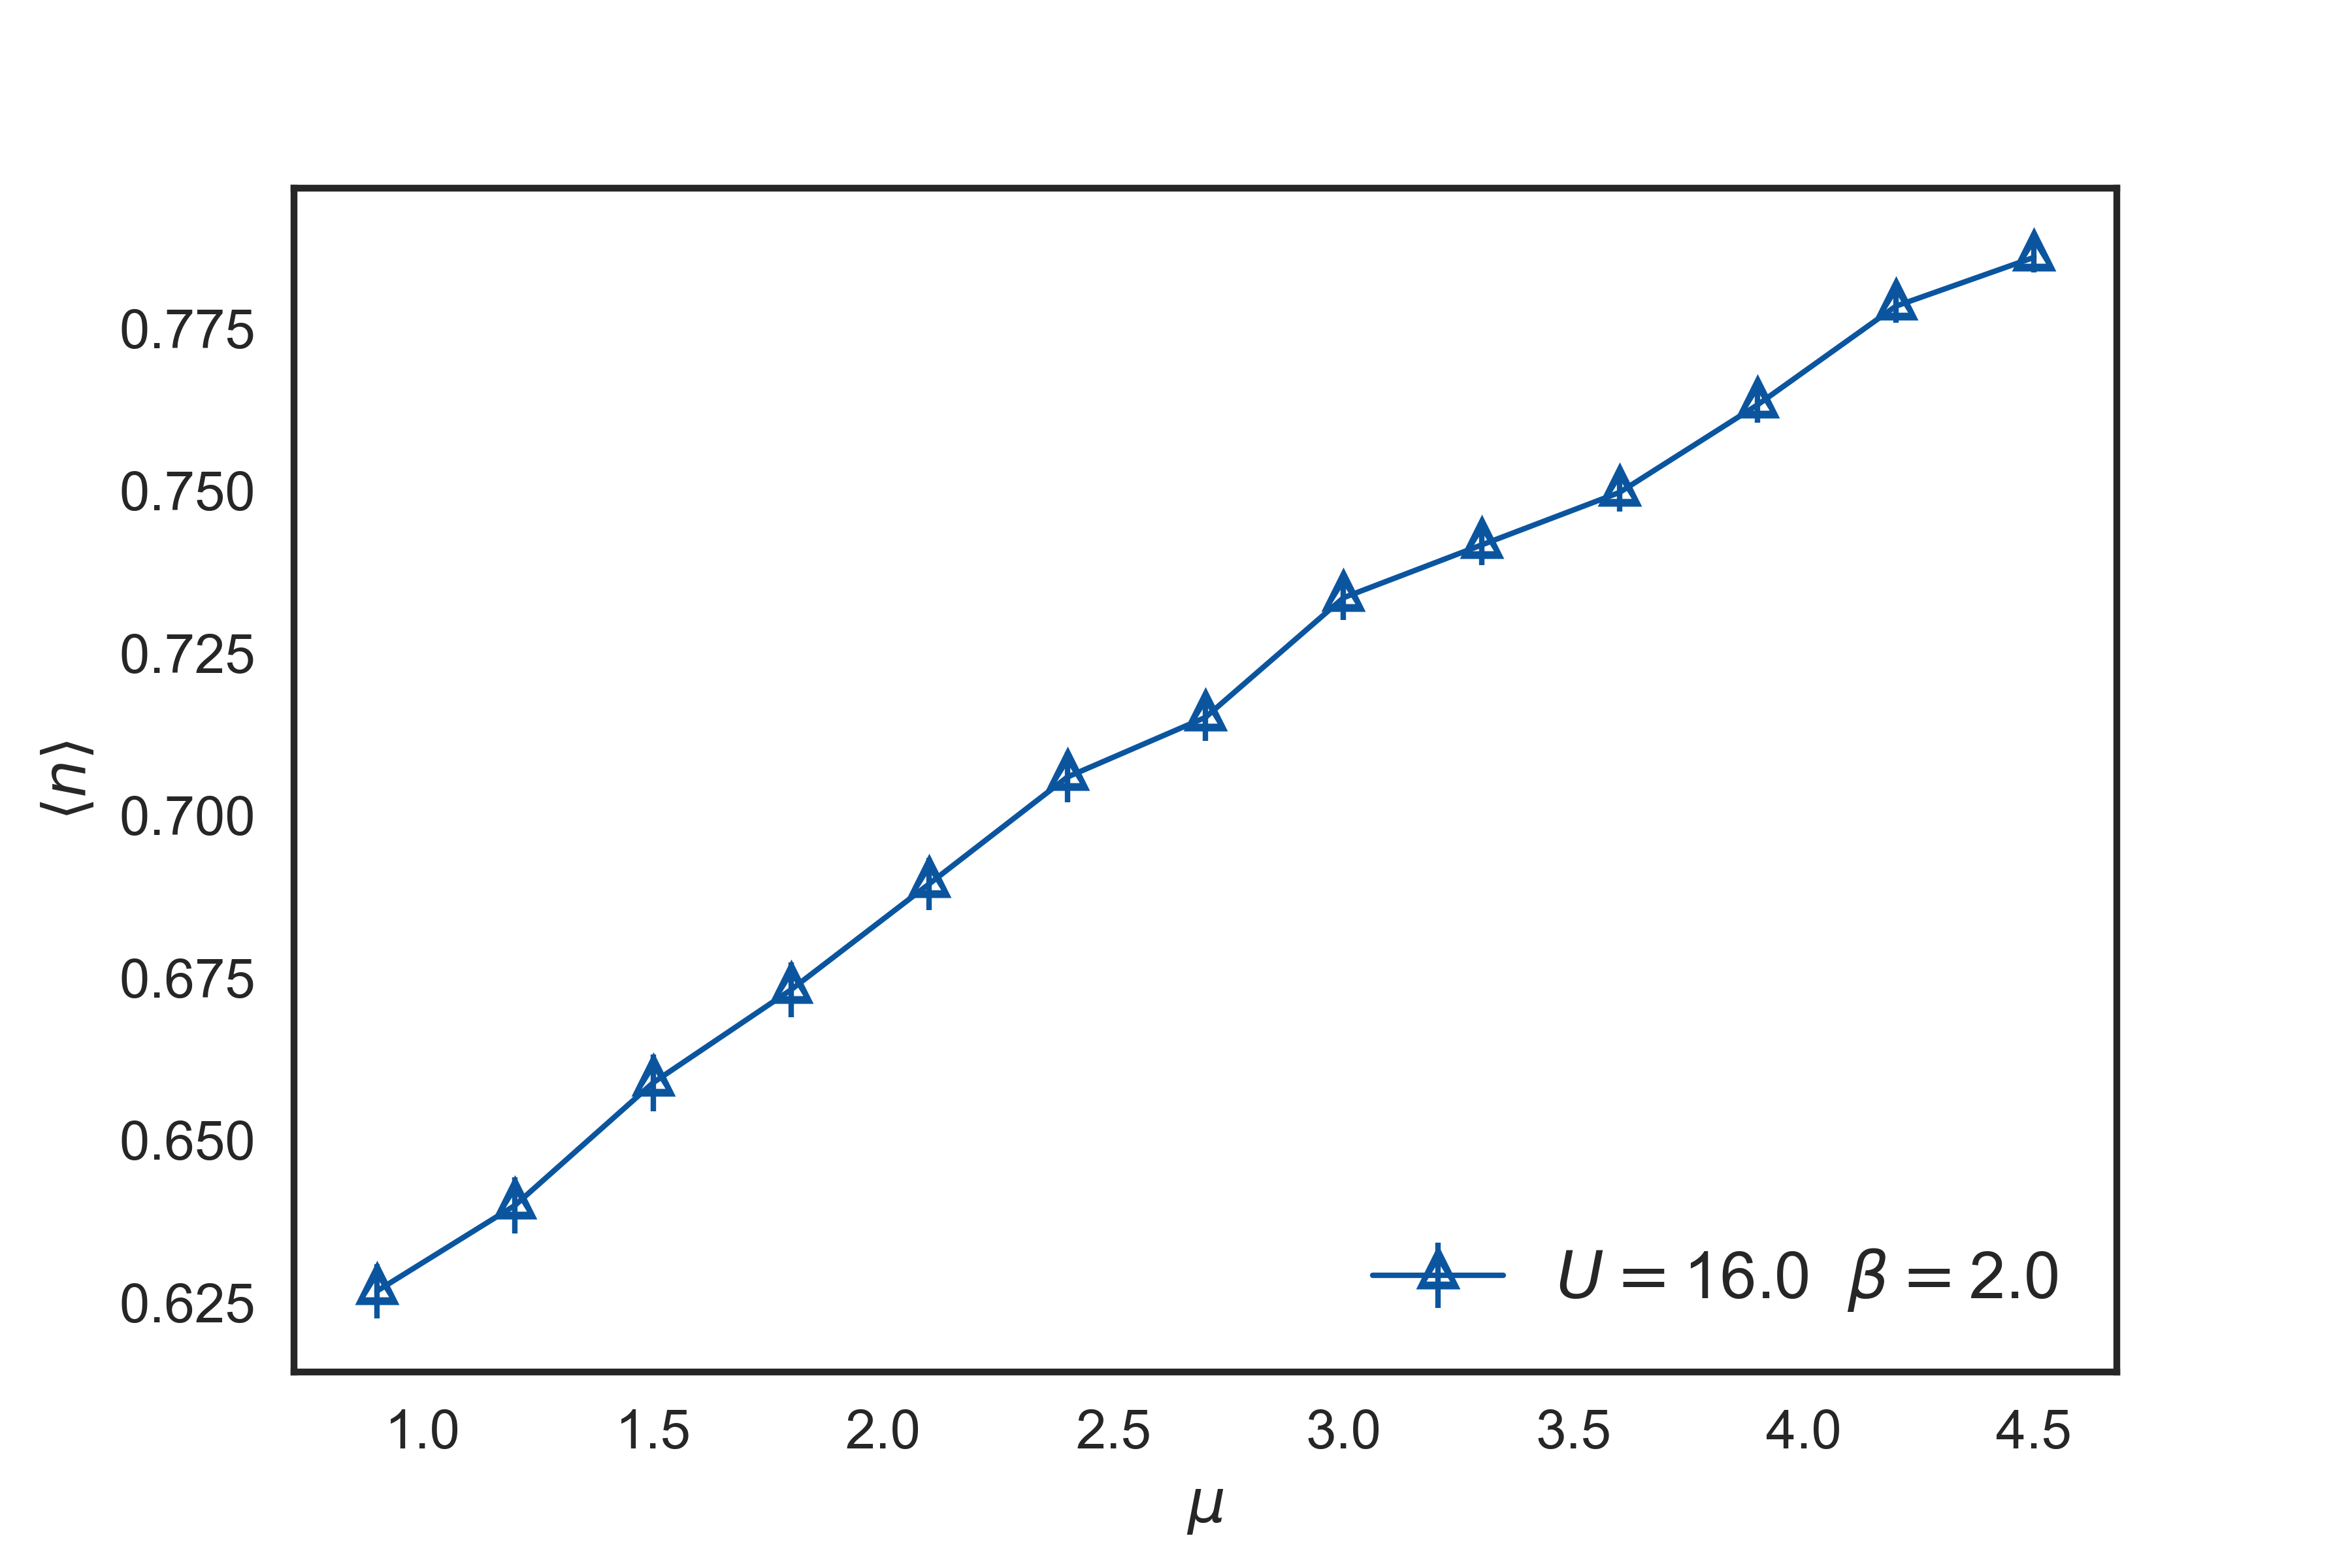
\includegraphics[scale = 0.5]{Applications/signTMDmusDensU16beta2.png}
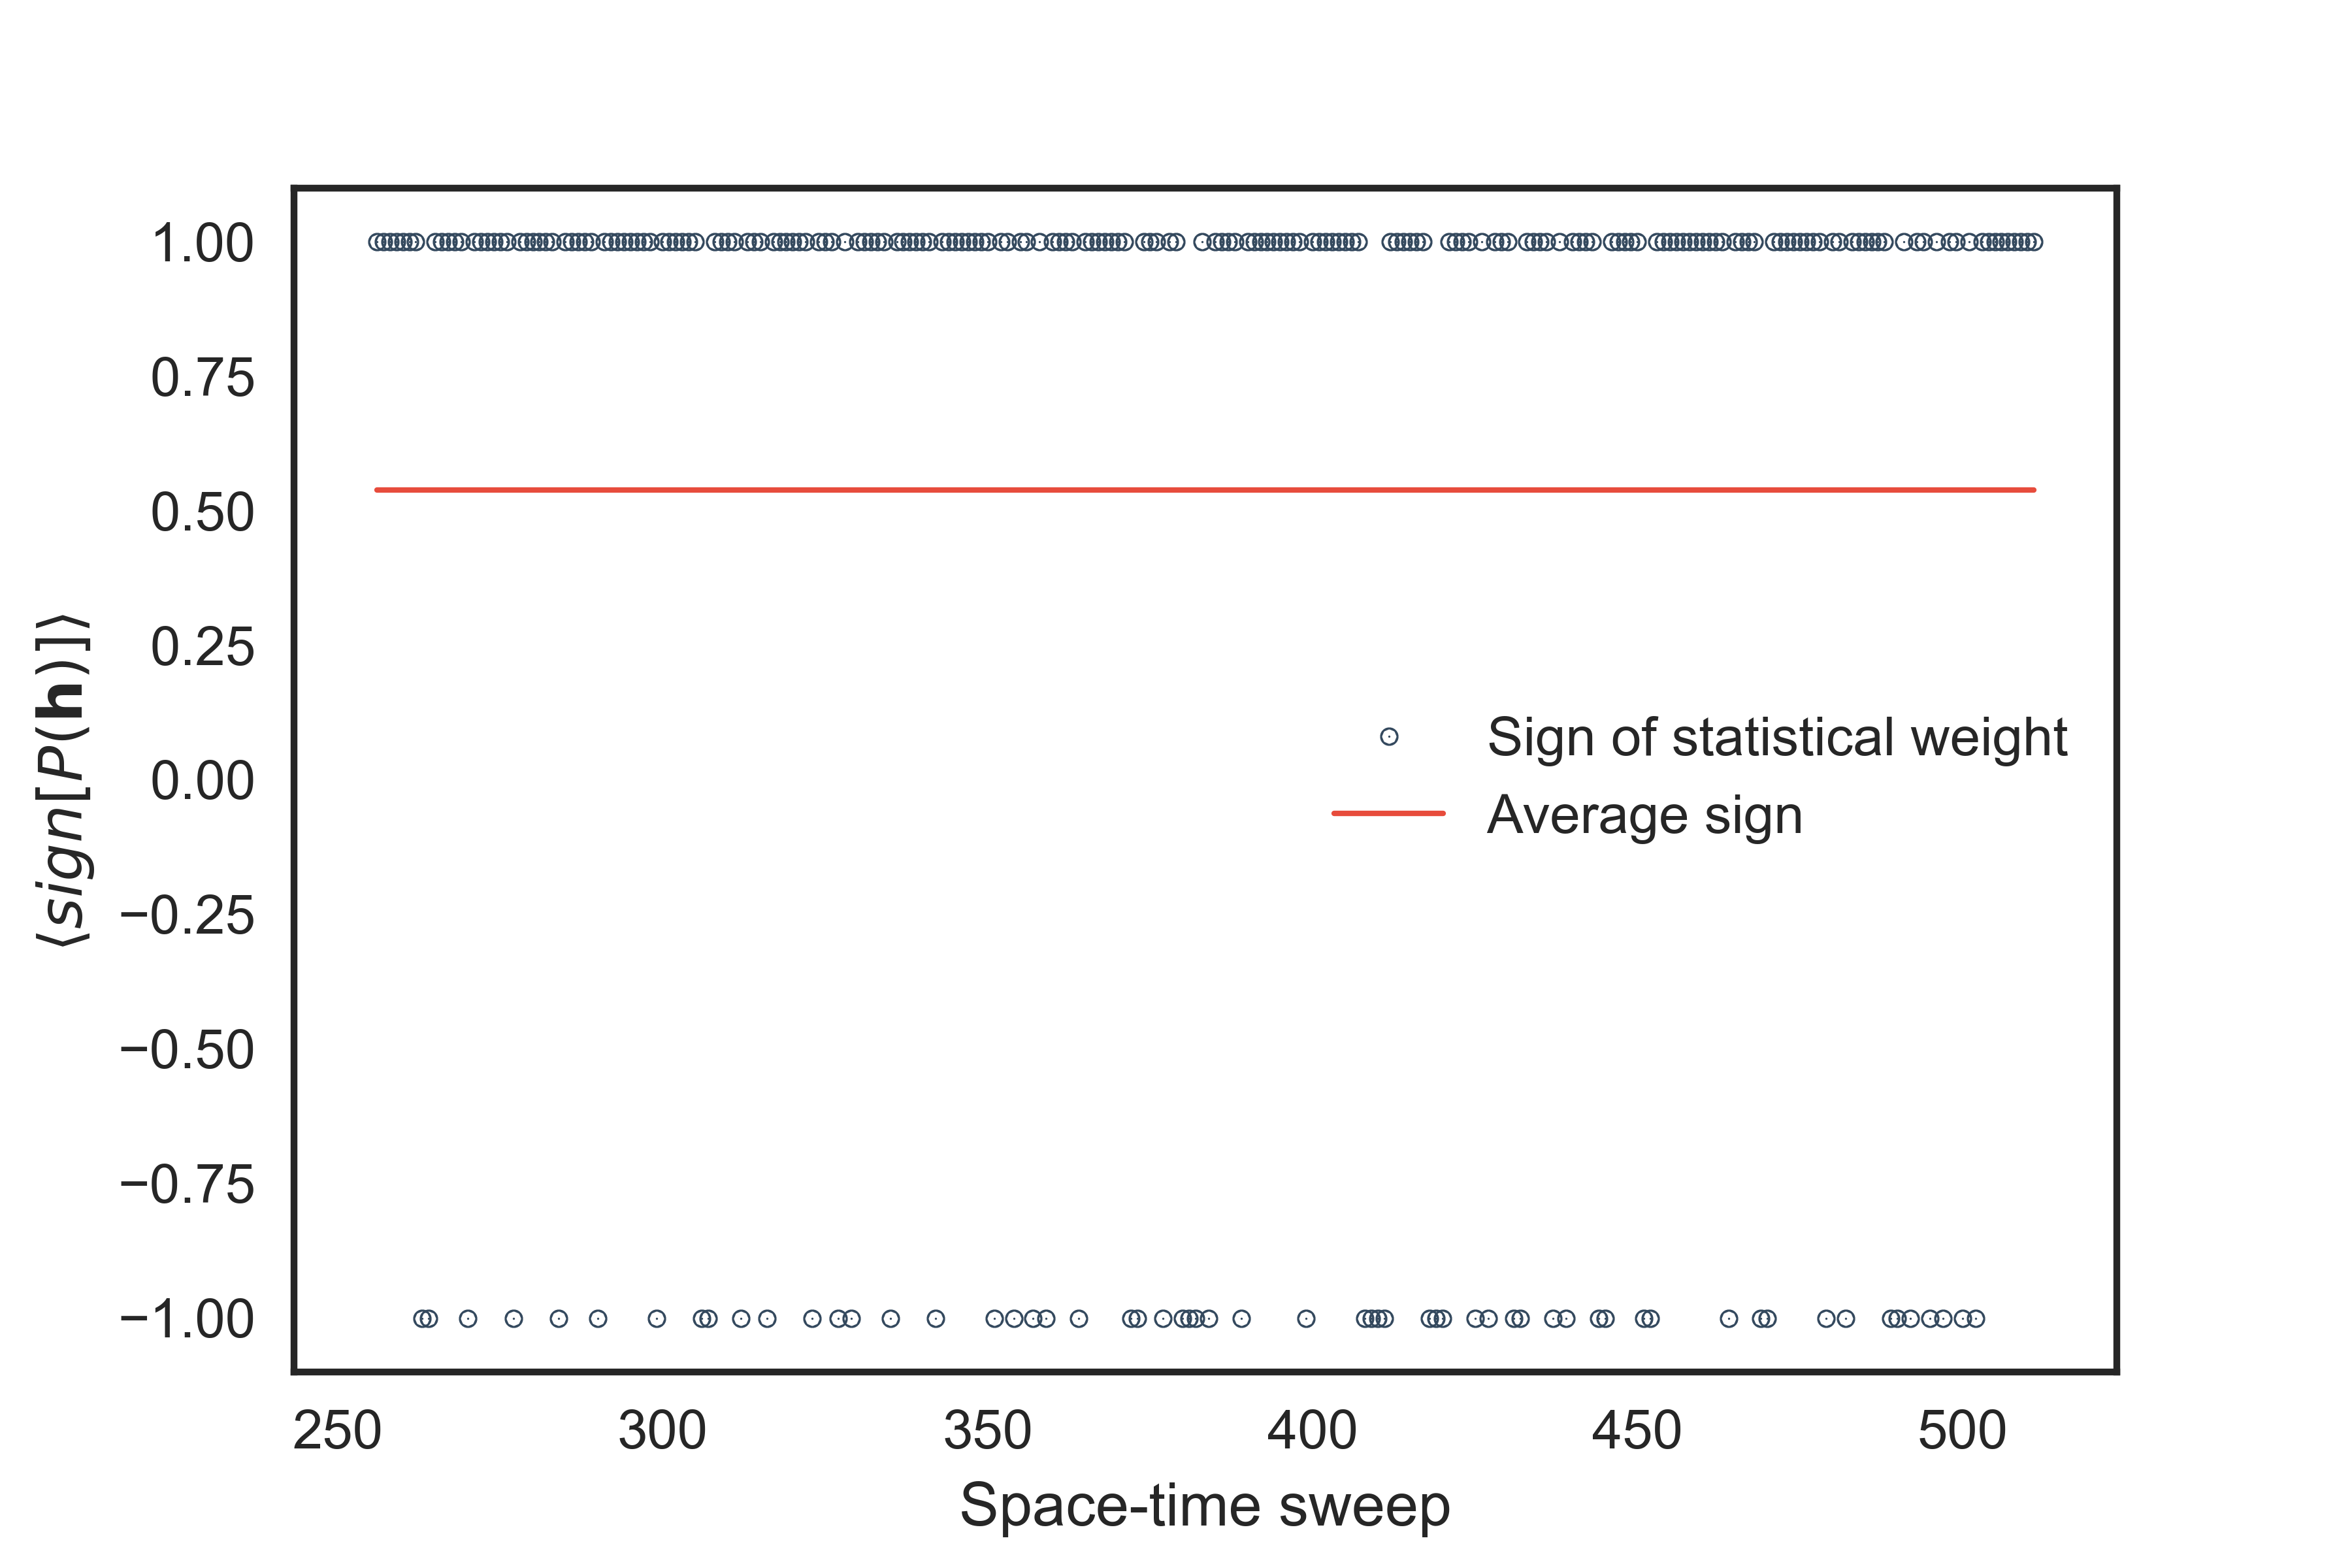
\includegraphics[scale = 0.5]{Applications/Local-av-sign.png}
	\caption[Electron density as a function of the chemical potential for the $9 \times 4$ \acs{TMD} nanoribbon, with $\beta = 2$ and $U = 16$. Sign of the accepted configuration as a function for a few space-time sweeps of the algorithm.]{Left: Electron density as a function of the chemical potential for the $9 \times 4$ \acs{TMD} nanoribbon, with $\beta = 2$ and $U = 16$.
	Right: Sign of the accepted configuration as a function for a few space-time sweeps of the algorithm, for the same \acs{TMDNR}; the red line is the local average of the sign.}
	\label{fig:SignLoc}
\end{figure}

To prove that the half filled square lattice is sign problem-free we start by invoking two well known identities.
Respectively, for any non-singular matrix $\bm A$, and for symmetric, non-singular matrices $\bm A_{l=1,... m}$:
\begin{equation}\label{eq:identities}
( \bm I + \bm A^{-1} )^{-1}  = \bm I - ( \bm I + \bm A )^{-1} \,\,\,\, \,\,\,\, ( \bm I + \bm A_m^{-1}  \bm A_{m-1}^{-1}  ...  \bm A_{1}^{-1} )^{-1} =  \bm I - [ ( \bm I + \bm A_m \bm A_{m-1} ... \bm A_1 )^{-1} ]^T
\end{equation}

Moreover, given any two matrices $\bm A$ and $\bm B$, there exists a third one $\bm \Pi$, which anti-commutes with $\bm A$, i.e. $ \bm \Pi \bm A  + \bm A \bm \Pi = 0$, and commutes with $\bm B$, i.e. $ \bm \Pi \bm B  - \bm B \bm \Pi = 0$ (or vice-versa).
Then, the following two relations hold:
\begin{equation}
\begin{split}
( \bm I + e^{\bm A - \bm B} )^{-1} &= \bm I - \bm \Pi^{-1} ( \bm I + e^{\bm A + \bm B} )^{-1} \bm \Pi \\
\det [ \bm I + e^{\bm A - \bm B} ] &= e^{\Tr [\bm A - \bm B ]} \det [ \bm I + e^{\bm A + \bm B} ]
\end{split}
\end{equation}

The first is proven by using the first identity of Eq.(\ref{eq:identities}):
\begin{equation}
\begin{split}
( \bm I + e^{\bm A - \bm B} )^{-1} &= \bm I - ( \bm I + e^{-\bm A + \bm B} )^{-1}  = \bm I - ( \bm I + e^{\bm \Pi^{-1} ( \bm A + \bm B) \bm \Pi } )^{-1} \\
&= \bm I - ( \bm I + \bm \Pi^{-1} e^{\bm A + \bm B} \bm \Pi )^{-1} = \bm I - \bm \Pi^{-1} ( \bm I + e^{\bm A + \bm B} )^{-1} \bm \Pi
\end{split}
\end{equation}

The proof of the second uses the commutation relations:
\begin{equation}
\begin{split}
\bm I + e^{\bm A - \bm B} &= e^{\bm A - \bm B} ( \bm I + e^{-(\bm A - \bm B)} ) = e^{\bm A - \bm B} ( \bm I + e^{-\bm A + \bm B} ) \\
&=e^{\bm A - \bm B} ( \bm I + e^{\bm \Pi^{-1} \bm A \bm \Pi +\bm \Pi^{-1} \bm B \bm \Pi  } ) = e^{\bm A - \bm B} ( \bm I + \bm \Pi^{-1} e^{\bm A + \bm B} \bm \Pi ) \\
&= e^{\bm A - \bm B}  \bm \Pi^{-1} ( \bm I + e^{\bm A + \bm B} ) \bm \Pi \\
\rightarrow \det [ \bm I + e^{\bm A - \bm B} ]&= \det [ e^{\bm A - \bm B} ] \det [ \bm \Pi^{-1} ] \det [ \bm I + e^{\bm A + \bm B} ] \det [ \bm \Pi ] \\
&= e^{ \Tr [ \bm A - \bm B ] } \det [ \bm I + e^{\bm A + \bm B} ]
\end{split}
\end{equation}

Similarly, we can prove that for symmetric matrices $\bm A$, $\bm B$, if we can find a non singular matrix $\bm \Pi$ that commutes with $\bm A$ and anti-commutes with $\bm B$, then:  $\det[ \bm I + e^{\bm A} e^{-\bm B} = e^{ \Tr [ \bm A - \bm B ] } \det [ \bm I + e^{\bm A} e^{\bm B} ]$ and
\begin{equation}
(\bm I + e^{\bm A} e^{-\bm B} )^{-1} = \bm I - [\bm \Pi^{-1}]^T [ ( \bm I + e^{\bm A} e^{\bm B} )^{-1} ]^T \bm [\bm \Pi^{-1} ]^T
\end{equation}

This theorem generalizes for the products we use in our code: $\bm M_\sigma = \bm I + e^{\bm A} e^{\sigma \bm B_k} e^{\bm A} e^{\sigma \bm B_{k-1}} ... e^{\bm A} e^{\sigma \bm B_1}$.
If we can find a non singular matrix $\bm \Pi$, such that $\{\bm \Pi, \bm A \} = 0$ and $[ \bm \Pi, \bm B_l] = 0$, then we have
\begin{equation}
\bm M_\downarrow^{-1} = \bm I -[ \bm \Pi^{-1}]^T [\bm M_\uparrow^{-1} ]^T \bm \Pi^T \quad \text{and} \quad \det [ \bm M_\downarrow ] = e^{k \Tr [ \bm A ] - \sum_{l = 1}^k \Tr [ \bm B_l] } \det [ \bm M_\uparrow ]
\end{equation}

Since $\det [ \bm M_\downarrow ] $ is then proportional to $\det [ \bm M_\uparrow ]$, and $e^{k \Tr [ \bm A ] - \sum_{l = 1}^k \Tr [ \bm B_l] }$ is positive, the weight of the classical spin configuration $\det [ \bm M_\uparrow ] \det [ \bm M_\downarrow ] $ will always be positive, and there will be no sign problem.
Now, it turns out that this is only possible at half filling.
Away from half filling, we cannot find a $\bm \Pi$ obeying these conditions.

The matrix $\bm \Pi$ is intimately related to the particle hole transformation.
In fact, for the \acs{1D} chain, or the square lattice, if we take $\bm \Pi_{x (y) } = \text{diag} ( 1, -1, 1, -1, ...)$, then the particle-hole transformation of the Green's function reads
\begin{equation}
\bm G^\downarrow = \bm I - \bm \Pi_x (\bm G^\uparrow)^T \bm \Pi_x \text{  for the chain} \,\, \text{and} \,\, \bm G^\downarrow = \bm I - \bm \Pi (\bm G^\uparrow)^T \bm \Pi \text{  for the square lattice} ,
\end{equation}
where $\bm \Pi = \bm \Pi_x \otimes \bm \Pi_y$, the tensor (Kronecker) product of the two matrices.

This reasoning is not only valid for the chain and square lattice, but actually holds for any bipartite lattice, such as the honeycomb lattice.
Unfortunately, for example for the triangular lattice, it does not.
This makes simulations on the triangular lattice (such as the one in this work) and other non bipartite lattices potentially much harder to control.